% Options for packages loaded elsewhere
% Options for packages loaded elsewhere
\PassOptionsToPackage{unicode}{hyperref}
\PassOptionsToPackage{hyphens}{url}
\PassOptionsToPackage{dvipsnames,svgnames,x11names}{xcolor}
%
\documentclass[
  spanish,
  letterpaper,
  DIV=11,
  numbers=noendperiod]{scrreprt}
\usepackage{xcolor}
\usepackage{amsmath,amssymb}
\setcounter{secnumdepth}{5}
\usepackage{iftex}
\ifPDFTeX
  \usepackage[T1]{fontenc}
  \usepackage[utf8]{inputenc}
  \usepackage{textcomp} % provide euro and other symbols
\else % if luatex or xetex
  \usepackage{unicode-math} % this also loads fontspec
  \defaultfontfeatures{Scale=MatchLowercase}
  \defaultfontfeatures[\rmfamily]{Ligatures=TeX,Scale=1}
\fi
\usepackage{lmodern}
\ifPDFTeX\else
  % xetex/luatex font selection
\fi
% Use upquote if available, for straight quotes in verbatim environments
\IfFileExists{upquote.sty}{\usepackage{upquote}}{}
\IfFileExists{microtype.sty}{% use microtype if available
  \usepackage[]{microtype}
  \UseMicrotypeSet[protrusion]{basicmath} % disable protrusion for tt fonts
}{}
\makeatletter
\@ifundefined{KOMAClassName}{% if non-KOMA class
  \IfFileExists{parskip.sty}{%
    \usepackage{parskip}
  }{% else
    \setlength{\parindent}{0pt}
    \setlength{\parskip}{6pt plus 2pt minus 1pt}}
}{% if KOMA class
  \KOMAoptions{parskip=half}}
\makeatother
% Make \paragraph and \subparagraph free-standing
\makeatletter
\ifx\paragraph\undefined\else
  \let\oldparagraph\paragraph
  \renewcommand{\paragraph}{
    \@ifstar
      \xxxParagraphStar
      \xxxParagraphNoStar
  }
  \newcommand{\xxxParagraphStar}[1]{\oldparagraph*{#1}\mbox{}}
  \newcommand{\xxxParagraphNoStar}[1]{\oldparagraph{#1}\mbox{}}
\fi
\ifx\subparagraph\undefined\else
  \let\oldsubparagraph\subparagraph
  \renewcommand{\subparagraph}{
    \@ifstar
      \xxxSubParagraphStar
      \xxxSubParagraphNoStar
  }
  \newcommand{\xxxSubParagraphStar}[1]{\oldsubparagraph*{#1}\mbox{}}
  \newcommand{\xxxSubParagraphNoStar}[1]{\oldsubparagraph{#1}\mbox{}}
\fi
\makeatother


\usepackage{longtable,booktabs,array}
\usepackage{calc} % for calculating minipage widths
% Correct order of tables after \paragraph or \subparagraph
\usepackage{etoolbox}
\makeatletter
\patchcmd\longtable{\par}{\if@noskipsec\mbox{}\fi\par}{}{}
\makeatother
% Allow footnotes in longtable head/foot
\IfFileExists{footnotehyper.sty}{\usepackage{footnotehyper}}{\usepackage{footnote}}
\makesavenoteenv{longtable}
\usepackage{graphicx}
\makeatletter
\newsavebox\pandoc@box
\newcommand*\pandocbounded[1]{% scales image to fit in text height/width
  \sbox\pandoc@box{#1}%
  \Gscale@div\@tempa{\textheight}{\dimexpr\ht\pandoc@box+\dp\pandoc@box\relax}%
  \Gscale@div\@tempb{\linewidth}{\wd\pandoc@box}%
  \ifdim\@tempb\p@<\@tempa\p@\let\@tempa\@tempb\fi% select the smaller of both
  \ifdim\@tempa\p@<\p@\scalebox{\@tempa}{\usebox\pandoc@box}%
  \else\usebox{\pandoc@box}%
  \fi%
}
% Set default figure placement to htbp
\def\fps@figure{htbp}
\makeatother



\ifLuaTeX
\usepackage[bidi=basic]{babel}
\else
\usepackage[bidi=default]{babel}
\fi
% get rid of language-specific shorthands (see #6817):
\let\LanguageShortHands\languageshorthands
\def\languageshorthands#1{}


\setlength{\emergencystretch}{3em} % prevent overfull lines

\providecommand{\tightlist}{%
  \setlength{\itemsep}{0pt}\setlength{\parskip}{0pt}}



 


\KOMAoption{captions}{tableheading}
\makeatletter
\@ifpackageloaded{tcolorbox}{}{\usepackage[skins,breakable]{tcolorbox}}
\@ifpackageloaded{fontawesome5}{}{\usepackage{fontawesome5}}
\definecolor{quarto-callout-color}{HTML}{909090}
\definecolor{quarto-callout-note-color}{HTML}{0758E5}
\definecolor{quarto-callout-important-color}{HTML}{CC1914}
\definecolor{quarto-callout-warning-color}{HTML}{EB9113}
\definecolor{quarto-callout-tip-color}{HTML}{00A047}
\definecolor{quarto-callout-caution-color}{HTML}{FC5300}
\definecolor{quarto-callout-color-frame}{HTML}{acacac}
\definecolor{quarto-callout-note-color-frame}{HTML}{4582ec}
\definecolor{quarto-callout-important-color-frame}{HTML}{d9534f}
\definecolor{quarto-callout-warning-color-frame}{HTML}{f0ad4e}
\definecolor{quarto-callout-tip-color-frame}{HTML}{02b875}
\definecolor{quarto-callout-caution-color-frame}{HTML}{fd7e14}
\makeatother
\makeatletter
\@ifpackageloaded{bookmark}{}{\usepackage{bookmark}}
\makeatother
\makeatletter
\@ifpackageloaded{caption}{}{\usepackage{caption}}
\AtBeginDocument{%
\ifdefined\contentsname
  \renewcommand*\contentsname{Tabla de contenidos}
\else
  \newcommand\contentsname{Tabla de contenidos}
\fi
\ifdefined\listfigurename
  \renewcommand*\listfigurename{Listado de Figuras}
\else
  \newcommand\listfigurename{Listado de Figuras}
\fi
\ifdefined\listtablename
  \renewcommand*\listtablename{Listado de Tablas}
\else
  \newcommand\listtablename{Listado de Tablas}
\fi
\ifdefined\figurename
  \renewcommand*\figurename{Figura}
\else
  \newcommand\figurename{Figura}
\fi
\ifdefined\tablename
  \renewcommand*\tablename{Tabla}
\else
  \newcommand\tablename{Tabla}
\fi
}
\@ifpackageloaded{float}{}{\usepackage{float}}
\floatstyle{ruled}
\@ifundefined{c@chapter}{\newfloat{codelisting}{h}{lop}}{\newfloat{codelisting}{h}{lop}[chapter]}
\floatname{codelisting}{Listado}
\newcommand*\listoflistings{\listof{codelisting}{Listado de Listados}}
\makeatother
\makeatletter
\makeatother
\makeatletter
\@ifpackageloaded{caption}{}{\usepackage{caption}}
\@ifpackageloaded{subcaption}{}{\usepackage{subcaption}}
\makeatother
\usepackage{bookmark}
\IfFileExists{xurl.sty}{\usepackage{xurl}}{} % add URL line breaks if available
\urlstyle{same}
\hypersetup{
  pdftitle={Notas de clase Business Analytics},
  pdfauthor={Daniel Parra},
  pdflang={es},
  colorlinks=true,
  linkcolor={blue},
  filecolor={Maroon},
  citecolor={Blue},
  urlcolor={Blue},
  pdfcreator={LaTeX via pandoc}}


\title{Notas de clase Business Analytics}
\author{Daniel Parra}
\date{Invalid Date}
\begin{document}
\maketitle

\renewcommand*\contentsname{Tabla de contenidos}
{
\hypersetup{linkcolor=}
\setcounter{tocdepth}{2}
\tableofcontents
}

\bookmarksetup{startatroot}

\chapter*{Bienvenidos}\label{bienvenidos}
\addcontentsline{toc}{chapter}{Bienvenidos}

\markboth{Bienvenidos}{Bienvenidos}

Este libro ha sido creado con el propósito de ofrecer un resumen claro y
conciso de los conceptos clave de las clases de Business Analytics para
los posgrados de administración de la Pontificia Universidad Javeriana.
Es un complemento diseñado para reforzar el aprendizaje en clase, pero
no pretende reemplazar la experiencia educativa que estas ofrecen.

Parte del texto en estas notas de clase ha sido elaborado con ayuda de
inteligencia artificial (ChatGPT), combinando apuntes propios y
referencias de diversos libros. Las ilustraciones, inspiradas en el
libro ``Math with Bad Drawings'' de Ben Orlin, también han sido
generadas utilizando inteligencia artificial.

© 2025 Pontificia Universidad Javeriana. Este libro está licenciado bajo
una licencia CC BY 4.0.

\bookmarksetup{startatroot}

\chapter{Introducción: Descubriendo la Analítica de
Datos}\label{introducciuxf3n-descubriendo-la-analuxedtica-de-datos}

Imagina que trabajas en una empresa que debe decidir qué producto lanzar
o qué precio poner a sus artículos. ¿Cómo tomas estas decisiones?
Antiguamente, las decisiones se tomaban según la intuición del jefe
(\textbf{HiPPO}, la persona mejor pagada en la organización), pero
actualmente contamos con algo mejor: la analítica de datos.

\section{¿Qué es la Analítica de Datos para
Negocios?}\label{quuxe9-es-la-analuxedtica-de-datos-para-negocios}

La analítica de datos es la aplicación de herramientas tecnológicas y
estadísticas para analizar información relevante y apoyar la toma de
decisiones en una organización.

Los datos, sin embargo, no son suficientes por sí solos. Necesitamos
interpretarlos de manera efectiva para contar historias convincentes que
permitan tomar decisiones informadas.

\section{¿Qué tipo de preguntas podemos responder con la
analítica?}\label{quuxe9-tipo-de-preguntas-podemos-responder-con-la-analuxedtica}

La analítica de negocios nos permite responder preguntas prácticas,
como:

\begin{itemize}
\tightlist
\item
  ¿Quiénes son mis clientes?
\item
  ¿Qué campaña de marketing es más efectiva?
\item
  ¿Cuál sería el efecto de cambiar los precios?
\item
  ¿Cómo predecir la demanda de un producto?
\end{itemize}

\section{Tipos de Analítica}\label{tipos-de-analuxedtica}

Hay tres tipos principales de analítica:

\subsection{Analítica Descriptiva}\label{analuxedtica-descriptiva}

Describe la situación actual mediante visualizaciones y estadísticas
básicas.

\textbf{Ejemplos:}

\begin{itemize}
\tightlist
\item
  ¿Han crecido las ventas este año?
\item
  ¿Qué región vende menos?
\end{itemize}

\subsection{Analítica Predictiva}\label{analuxedtica-predictiva}

Predice qué sucederá, aprovechando correlaciones entre variables. Aquí
no es necesaria la causalidad, sino una relación estadística sólida.

\textbf{Ejemplos:}

\begin{itemize}
\tightlist
\item
  ¿Cuál es la probabilidad de que un cliente deje de comprar?
\item
  ¿Qué tan probable es que una transacción sea fraudulenta?
\end{itemize}

\subsection{Analítica Prescriptiva}\label{analuxedtica-prescriptiva}

Sugiere decisiones óptimas, enfocándose en relaciones causales y,
frecuentemente, utilizando experimentos.

\textbf{Ejemplos:}

\begin{itemize}
\tightlist
\item
  ¿Subir el precio incrementará las ganancias?
\item
  ¿Qué diseño de página web aumentará las ventas?
\end{itemize}

\section{La cadena de valor en Business
Analytics}\label{la-cadena-de-valor-en-business-analytics}

La analítica de negocios incluye:

\begin{itemize}
\tightlist
\item
  \textbf{Recolección y organización de datos:} Crear bases de datos
  (SQL, Power BI).
\item
  \textbf{Análisis de datos:} Usar herramientas como R, Excel o Python
  para análisis estratégicos.
\item
  \textbf{Comunicación de resultados:} Presentar hallazgos en reportes y
  visualizaciones (PowerPoint, Tableau, Quarto).
\end{itemize}

\bookmarksetup{startatroot}

\chapter{Fundamentos de Variables y Visualización de
Datos}\label{fundamentos-de-variables-y-visualizaciuxf3n-de-datos}

\section{Introducción a Variables y
Datos}\label{introducciuxf3n-a-variables-y-datos}

Antes de manipular o graficar, es importante entender qué son los datos
y las variables.

\begin{tcolorbox}[enhanced jigsaw, arc=.35mm, leftrule=.75mm, colbacktitle=quarto-callout-note-color!10!white, left=2mm, opacitybacktitle=0.6, toptitle=1mm, title=\textcolor{quarto-callout-note-color}{\faInfo}\hspace{0.5em}{Definiciones clave}, colframe=quarto-callout-note-color-frame, toprule=.15mm, colback=white, rightrule=.15mm, opacityback=0, coltitle=black, breakable, bottomtitle=1mm, titlerule=0mm, bottomrule=.15mm]

\begin{itemize}
\tightlist
\item
  \textbf{Variable:} Característica que puede cambiar entre
  observaciones (ej. género, ventas, PIB).\\
\item
  \textbf{Datos:} Conjunto de observaciones (filas) con valores para
  esas variables (columnas).
\end{itemize}

\end{tcolorbox}

\subsection{Tipos de variables}\label{tipos-de-variables}

Las variables se clasifican en dos grandes categorías según su
naturaleza:

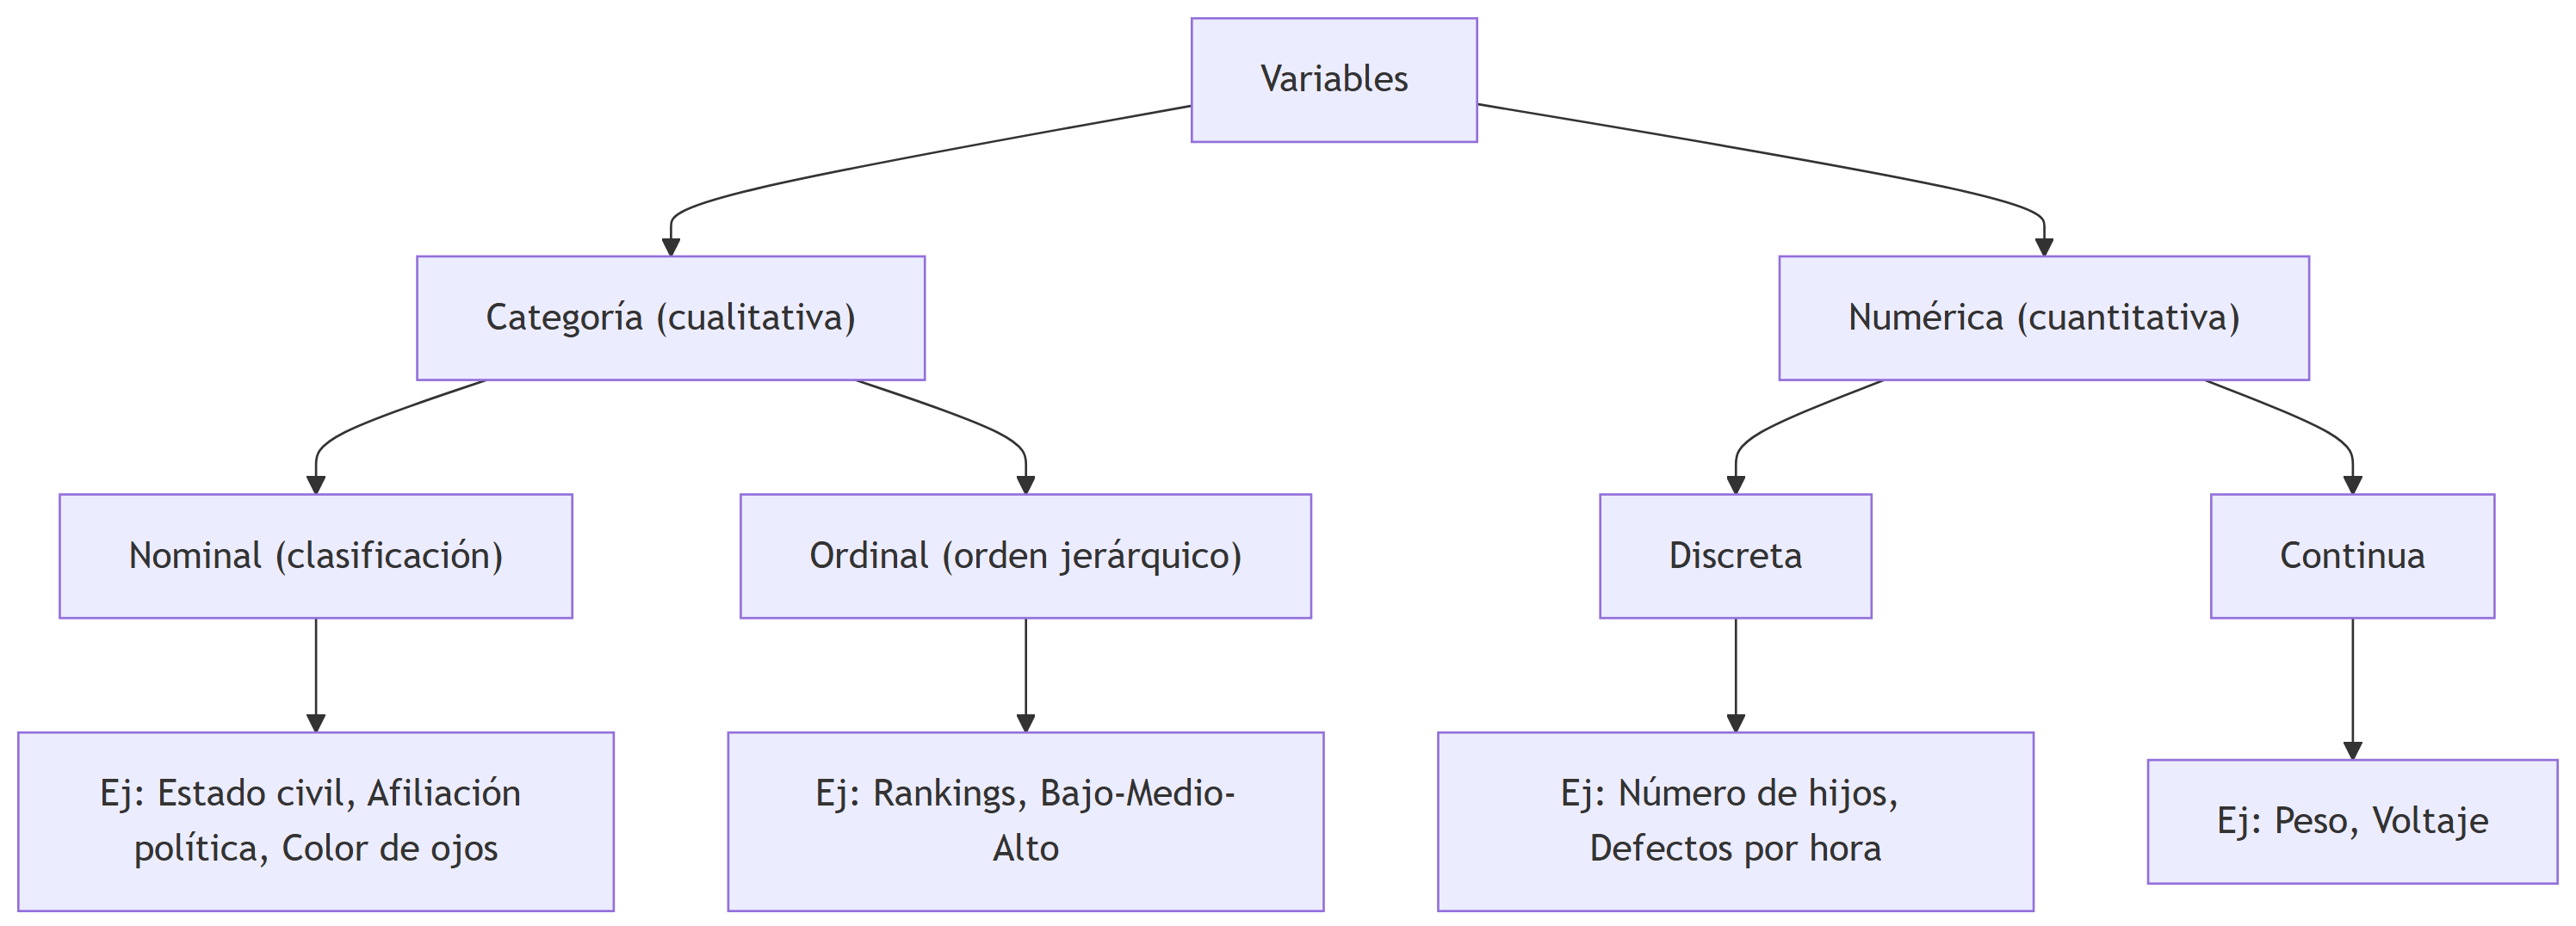
\includegraphics[width=11.72in,height=4.23in]{capitulo2_files/figure-latex/mermaid-figure-1.png}

Clasificación de Variables

Entender el tipo de variable es clave porque:

\begin{itemize}
\tightlist
\item
  \textbf{Define el resumen estadístico adecuado:} No calculamos una
  media de colores de ojos.\\
\item
  \textbf{Determina el gráfico apropiado:} Un histograma para variables
  numéricas, un gráfico de barras para categorías.\\
\item
  \textbf{Evita errores de interpretación:} Un ordinal tratado como
  numérico puede dar conclusiones equivocadas.
\end{itemize}

Ejemplos de tipos de variables:

\begin{longtable}[]{@{}
  >{\raggedright\arraybackslash}p{(\linewidth - 4\tabcolsep) * \real{0.4924}}
  >{\raggedright\arraybackslash}p{(\linewidth - 4\tabcolsep) * \real{0.3258}}
  >{\raggedright\arraybackslash}p{(\linewidth - 4\tabcolsep) * \real{0.1818}}@{}}
\caption{Ejemplo: Tipos de Variables en una
Encuesta}\label{tbl-ejemplos}\tabularnewline
\toprule\noalign{}
\begin{minipage}[b]{\linewidth}\raggedright
Pregunta
\end{minipage} & \begin{minipage}[b]{\linewidth}\raggedright
Respuesta
\end{minipage} & \begin{minipage}[b]{\linewidth}\raggedright
Tipo de Variable
\end{minipage} \\
\midrule\noalign{}
\endfirsthead
\toprule\noalign{}
\begin{minipage}[b]{\linewidth}\raggedright
Pregunta
\end{minipage} & \begin{minipage}[b]{\linewidth}\raggedright
Respuesta
\end{minipage} & \begin{minipage}[b]{\linewidth}\raggedright
Tipo de Variable
\end{minipage} \\
\midrule\noalign{}
\endhead
\bottomrule\noalign{}
\endlastfoot
¿Tiene perfil de Facebook? & Sí / No & Categórica Nominal \\
¿Cuántos mensajes de texto ha enviado en los últimos dos días? &
\_\_\_\_\_\_\_\_ (número entero) & Numérica Discreta \\
¿Cuánto tiempo le tomó bajar la aplicación? & \_\_\_\_\_\_\_\_ (minutos
o segundos) & Numérica Continua \\
¿Cómo evaluaría su experiencia en Facebook? & Muy mala, Mala, Regular,
Buena, Muy buena & Categórica Ordinal \\
\end{longtable}

\section{Organización de Datos
Categóricos}\label{organizaciuxf3n-de-datos-categuxf3ricos}

\subsection{Tablas para Datos
Categóricos}\label{tablas-para-datos-categuxf3ricos}

\textbf{Tabla resumen:} Muestra frecuencias o porcentajes para cada
categoría de la variable. A continuación mostramos cómo se distribuyen
las calificaciones de nuestro restaurante en Google Maps, basadas en 100
reseñas:

\begin{longtable}[]{@{}lcc@{}}
\caption{Resumen de Calificaciones en Google
Maps}\label{tbl-calificaciones}\tabularnewline
\toprule\noalign{}
Calificación & Frecuencia & \% sobre 100 reseñas \\
\midrule\noalign{}
\endfirsthead
\toprule\noalign{}
Calificación & Frecuencia & \% sobre 100 reseñas \\
\midrule\noalign{}
\endhead
\bottomrule\noalign{}
\endlastfoot
Excelente & 40 & 40\% \\
Buena & 35 & 35\% \\
Regular & 20 & 20\% \\
Mala & 5 & 5\% \\
\end{longtable}

\textbf{Tabla de contingencia:} Relaciona dos o más variables
categóricas. Muestra la frecuencia con la que ocurren combinaciones de
categorías. Por ejemplo, las calificaciones según la hora del día:

\begin{longtable}[]{@{}
  >{\raggedright\arraybackslash}p{(\linewidth - 8\tabcolsep) * \real{0.1750}}
  >{\centering\arraybackslash}p{(\linewidth - 8\tabcolsep) * \real{0.2000}}
  >{\centering\arraybackslash}p{(\linewidth - 8\tabcolsep) * \real{0.2000}}
  >{\centering\arraybackslash}p{(\linewidth - 8\tabcolsep) * \real{0.2000}}
  >{\centering\arraybackslash}p{(\linewidth - 8\tabcolsep) * \real{0.2250}}@{}}
\caption{Calificaciones por Hora del
Día}\label{tbl-contingencia}\tabularnewline
\toprule\noalign{}
\begin{minipage}[b]{\linewidth}\raggedright
Calificación
\end{minipage} & \begin{minipage}[b]{\linewidth}\centering
Mañana (n, \%)
\end{minipage} & \begin{minipage}[b]{\linewidth}\centering
Tarde (n, \%)
\end{minipage} & \begin{minipage}[b]{\linewidth}\centering
Noche (n, \%)
\end{minipage} & \begin{minipage}[b]{\linewidth}\centering
Madrugada (n, \%)
\end{minipage} \\
\midrule\noalign{}
\endfirsthead
\toprule\noalign{}
\begin{minipage}[b]{\linewidth}\raggedright
Calificación
\end{minipage} & \begin{minipage}[b]{\linewidth}\centering
Mañana (n, \%)
\end{minipage} & \begin{minipage}[b]{\linewidth}\centering
Tarde (n, \%)
\end{minipage} & \begin{minipage}[b]{\linewidth}\centering
Noche (n, \%)
\end{minipage} & \begin{minipage}[b]{\linewidth}\centering
Madrugada (n, \%)
\end{minipage} \\
\midrule\noalign{}
\endhead
\bottomrule\noalign{}
\endlastfoot
Excelente & 10 (40\%) & 15 (50\%) & 10 (33.3\%) & 5 (62.5\%) \\
Buena & 8 (32\%) & 10 (33.3\%) & 8 (26.7\%) & 2 (25\%) \\
Regular & 4 (16\%) & 3 (10\%) & 7 (23.3\%) & 1 (12.5\%) \\
Mala & 3 (12\%) & 2 (6.7\%) & 5 (16.7\%) & 0 (0\%) \\
\textbf{Total} & \textbf{25 (100\%)} & \textbf{30 (100\%)} & \textbf{30
(100\%)} & \textbf{8 (100\%)} \\
\end{longtable}

Al analizar la tabla de contingencia, podemos comparar cómo varían las
calificaciones según la hora del día. Por ejemplo, la madrugada muestra
un 62.5\% de reseñas ``Excelente'' y ninguna ``Mala'', lo que sugiere
que quienes califican en ese horario son clientes muy satisfechos
(posiblemente menos volumen y mejor atención). En cambio, durante la
noche la proporción de calificaciones ``Excelente'' baja a 33.3\% y
aumentan las ``Mala'' (16.7\%), lo que podría indicar saturación
operativa o tiempos de espera más largos.

La tarde destaca por concentrar el mayor número de reseñas totales y un
50\% de valoraciones ``Excelente'', lo que la convierte en una franja
estratégica para mantener estándares altos. Estos patrones permiten
priorizar recursos: reforzar personal nocturno y replicar buenas
prácticas de la madrugada y la tarde.

\subsection{Visualizando datos
categóricos}\label{visualizando-datos-categuxf3ricos}

\subsubsection{Gráfico de Barras}\label{gruxe1fico-de-barras}

Los gráficos de barras son la herramienta más versátil para visualizar
variables categóricas. Utilizan barras rectangulares cuya longitud (o
altura) es proporcional a la frecuencia o porcentaje de cada categoría.
Su principal ventaja es la facilidad para comparar visualmente
diferentes categorías, ya que el ojo humano puede detectar rápidamente
diferencias en longitud.

Las barras pueden orientarse vertical u horizontalmente, y son
especialmente útiles cuando los nombres de las categorías son largos
(mejor horizontal) o cuando queremos enfatizar el orden jerárquico de
los valores (mejor vertical). A diferencia de otros gráficos, las barras
deben comenzar siempre desde cero para no distorsionar las comparaciones
visuales. Mira un ejemplo de gráfico de barras:

\begin{figure}

\centering{

\pandocbounded{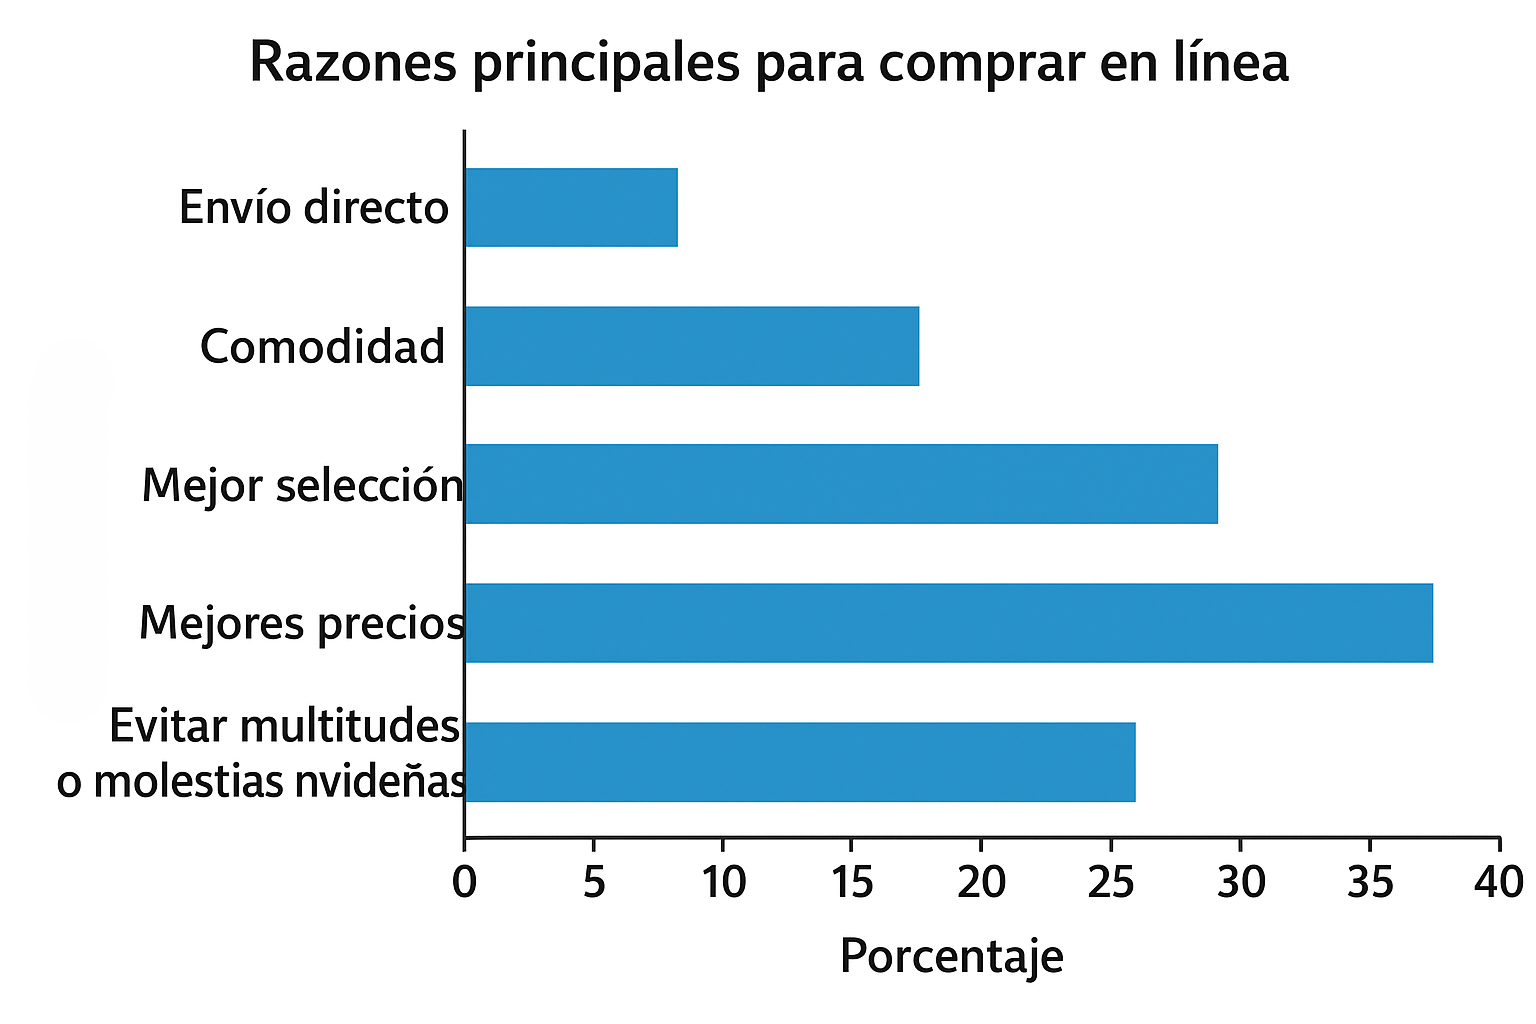
\includegraphics[keepaspectratio]{img/bar_chart.png}}

}

\caption{\label{fig-bar-chart}Ejemplo de gráfico de barras mostrando la
distribución de calificaciones}

\end{figure}%

\subsubsection{Gráfico de Torta (Pie
Chart)}\label{gruxe1fico-de-torta-pie-chart}

Los gráficos de torta representan datos categóricos como sectores de un
círculo, donde cada sector es proporcional al porcentaje que representa
esa categoría del total. La ``torta'' completa suma siempre 100\%, y
cada ``rebanada'' muestra visualmente qué proporción ocupa cada
categoría.

Su principal fortaleza es mostrar la \textbf{composición del total} - es
decir, cómo se distribuye un todo entre sus partes. Son especialmente
útiles cuando queremos enfatizar que una categoría domina sobre las
demás o cuando la pregunta clave es ``¿qué porcentaje del total
representa cada grupo?''. Por ejemplo, para mostrar la participación de
mercado de diferentes marcas o la distribución del presupuesto entre
departamentos. Este sería el gráfico de torta que muestra la misma
información del gráfico de barras anterior:

\begin{figure}

\centering{

\pandocbounded{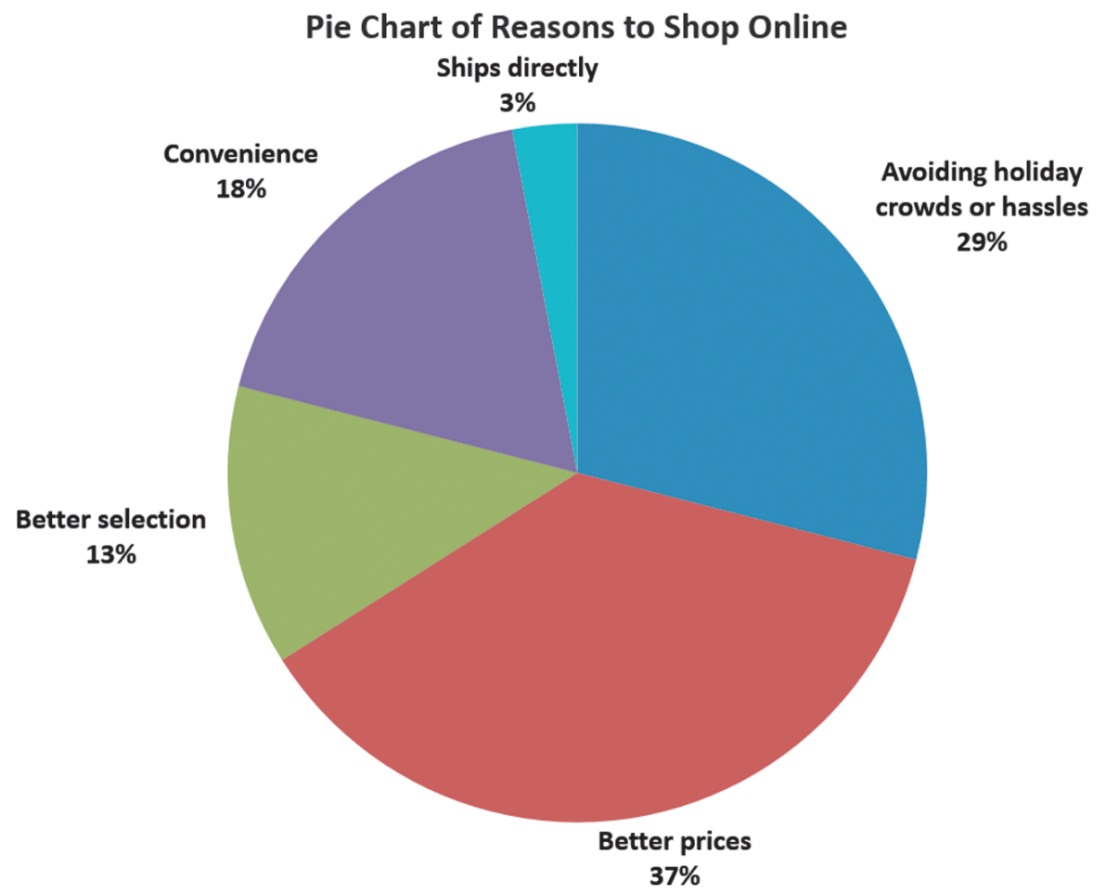
\includegraphics[keepaspectratio]{img/pie.png}}

}

\caption{\label{fig-pie-chart}Ejemplo de gráfico de torta mostrando la
distribución de calificaciones}

\end{figure}%

\begin{tcolorbox}[enhanced jigsaw, arc=.35mm, leftrule=.75mm, colbacktitle=quarto-callout-warning-color!10!white, left=2mm, opacitybacktitle=0.6, toptitle=1mm, title=\textcolor{quarto-callout-warning-color}{\faExclamationTriangle}\hspace{0.5em}{Limitaciones del gráfico de torta}, colframe=quarto-callout-warning-color-frame, toprule=.15mm, colback=white, rightrule=.15mm, opacityback=0, coltitle=black, breakable, bottomtitle=1mm, titlerule=0mm, bottomrule=.15mm]

\begin{itemize}
\tightlist
\item
  \textbf{Difícil comparación de sectores similares:} El ojo humano no
  distingue bien diferencias pequeñas entre ángulos
\item
  \textbf{Máximo recomendado:} No más de 5-7 categorías para mantener
  legibilidad
\item
  \textbf{Mejor alternativa:} Considera un gráfico de barras si
  necesitas comparar categorías con valores muy cercanos
\end{itemize}

\end{tcolorbox}

Los gráficos de torta funcionan mejor cuando hay una o dos categorías
claramente dominantes y el resto son minoritarias. Si todas las
categorías tienen tamaños similares, un gráfico de barras será más
efetorctivo para la comparación visual.

\subsubsection{Gráfico de Pareto}\label{gruxe1fico-de-pareto}

El gráfico de Pareto combina barras y una línea para identificar las
categorías más importantes según el \textbf{principio de Pareto} (regla
80-20). Las barras muestran las frecuencias ordenadas de mayor a menor,
mientras que la línea representa el porcentaje acumulado hasta llegar al
100\%.

Su objetivo principal es \textbf{priorizar} - ayuda a identificar las
pocas categorías que concentran la mayor parte del problema o fenómeno.
Por ejemplo, en control de calidad, unas pocas causas suelen generar la
mayoría de los defectos; en ventas, unos pocos productos pueden generar
la mayor parte de los ingresos.

\textbf{Elementos clave del gráfico de Pareto:}

\begin{itemize}
\tightlist
\item
  \textbf{Barras ordenadas:} De mayor a menor frecuencia (izquierda a
  derecha)
\item
  \textbf{Línea acumulada:} Muestra el porcentaje que suman las
  categorías hasta ese punto
\item
  \textbf{Principio 80-20:} Busca el punto donde pocas categorías
  explican la mayoría del fenómeno
\end{itemize}

\begin{figure}

\centering{

\pandocbounded{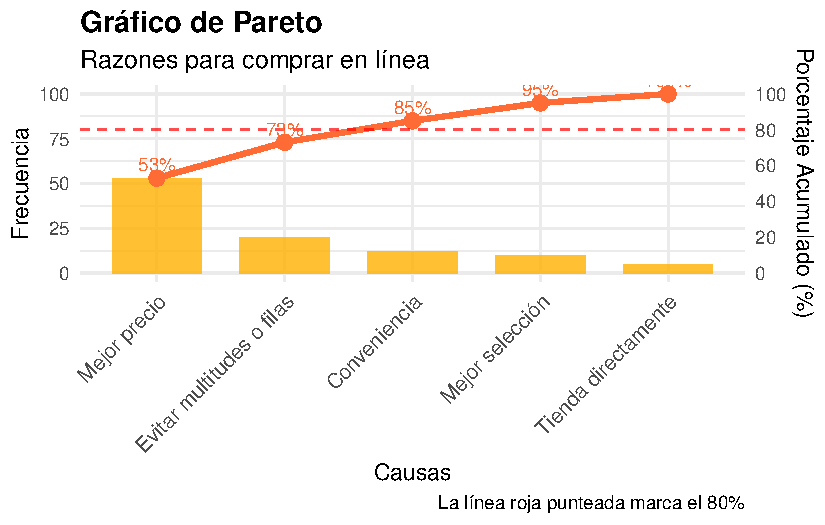
\includegraphics[keepaspectratio]{capitulo2_files/figure-pdf/fig-pareto-chart-1.pdf}}

}

\caption{\label{fig-pareto-chart}Gráfico de Pareto - Análisis de Causas
de Defectos}

\end{figure}%

\begin{tcolorbox}[enhanced jigsaw, arc=.35mm, leftrule=.75mm, colbacktitle=quarto-callout-tip-color!10!white, left=2mm, opacitybacktitle=0.6, toptitle=1mm, title=\textcolor{quarto-callout-tip-color}{\faLightbulb}\hspace{0.5em}{¿Cuándo usar un gráfico de Pareto?}, colframe=quarto-callout-tip-color-frame, toprule=.15mm, colback=white, rightrule=.15mm, opacityback=0, coltitle=black, breakable, bottomtitle=1mm, titlerule=0mm, bottomrule=.15mm]

\begin{itemize}
\tightlist
\item
  \textbf{Identificar prioridades:} ¿Qué problemas atender primero?
\item
  \textbf{Análisis de causas:} ¿Qué factores tienen mayor impacto?
\item
  \textbf{Optimización de recursos:} ¿Dónde enfocar los esfuerzos?
\item
  \textbf{Seguimiento de mejoras:} ¿Las acciones redujeron las causas
  principales?
\end{itemize}

\end{tcolorbox}

\textbf{Ejemplo práctico:} Si analizamos las quejas de un restaurante y
encontramos que ``comida fría'' y ``tiempo de espera'' representan el
75\% de todas las quejas, sabemos que resolver estos dos problemas
tendrá el mayor impacto en la satisfacción del cliente. El gráfico de
Pareto haría visible esta concentración de manera inmediata.

\subsection{Visualizando datos categóricos: Gráfico de Barras
Emparejadas}\label{visualizando-datos-categuxf3ricos-gruxe1fico-de-barras-emparejadas}

El \textbf{gráfico de barras emparejadas} (o agrupadas) se utiliza
cuando queremos comparar cómo se distribuye una variable categórica
principal dentro de los niveles de otra variable categórica. Cada grupo
del eje horizontal representa una categoría de la primera variable y,
dentro de cada grupo, las barras muestran las categorías de la segunda.

\textbf{Ejemplo:} Si analizamos las calificaciones de un restaurante
(Excelente, Buena, Regular, Mala) según la hora del día en que se dejó
la reseña (Mañana, Tarde, Noche), podemos ver rápidamente en qué horario
se concentran más las opiniones positivas.\\
Este tipo de gráfico ayuda a detectar patrones de comparación entre
grupos: diferencias claras en alturas de barras indican posibles áreas
de mejora o fortalezas.

\begin{figure}

\centering{

\pandocbounded{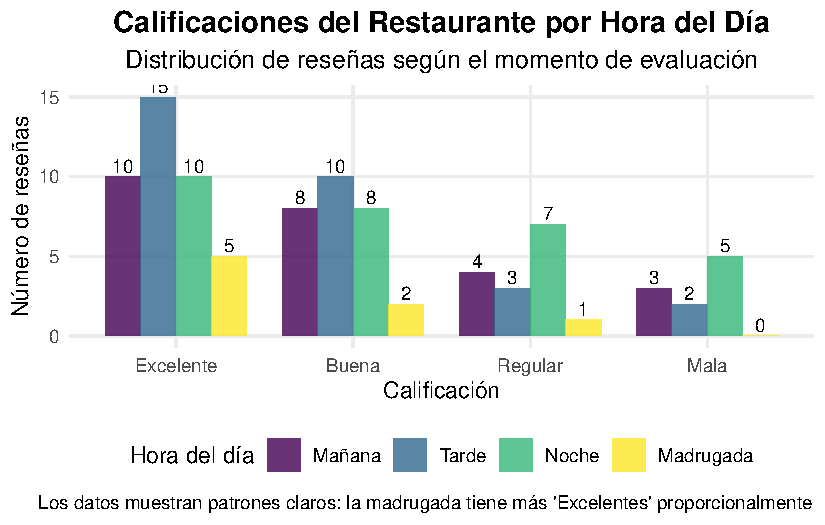
\includegraphics[keepaspectratio]{capitulo2_files/figure-pdf/fig-grouped-bars-1.pdf}}

}

\caption{\label{fig-grouped-bars}Gráfico de Barras Emparejadas -
Calificaciones por Hora del Día}

\end{figure}%

\textbf{Cuándo usarlo:}

\begin{itemize}
\tightlist
\item
  Cuando tienes \textbf{dos variables categóricas}.
\item
  Para comparar proporciones o frecuencias entre subgrupos.
\item
  Como complemento visual de una tabla de contingencia.
\end{itemize}

\textbf{Recomendaciones:}

\begin{itemize}
\tightlist
\item
  Ordena las categorías de forma lógica (por tiempo, intensidad, etc.).
\item
  Usa una leyenda clara.
\item
  Evita el exceso de colores; prioriza el contraste.
\end{itemize}

En resumen: antes de elegir cómo mostrar tus datos categóricos, conviene
pensar cuántas variables estás analizando. El siguiente esquema resume
las opciones más comunes: si trabajas con una sola variable, puedes
resumirla con una tabla y luego elegir un gráfico de barras, de torta o
de Pareto según el objetivo. Si tienes dos variables categóricas, una
tabla de contingencia es el punto de partida y suele representarse con
un gráfico de barras emparejadas para comparar grupos.

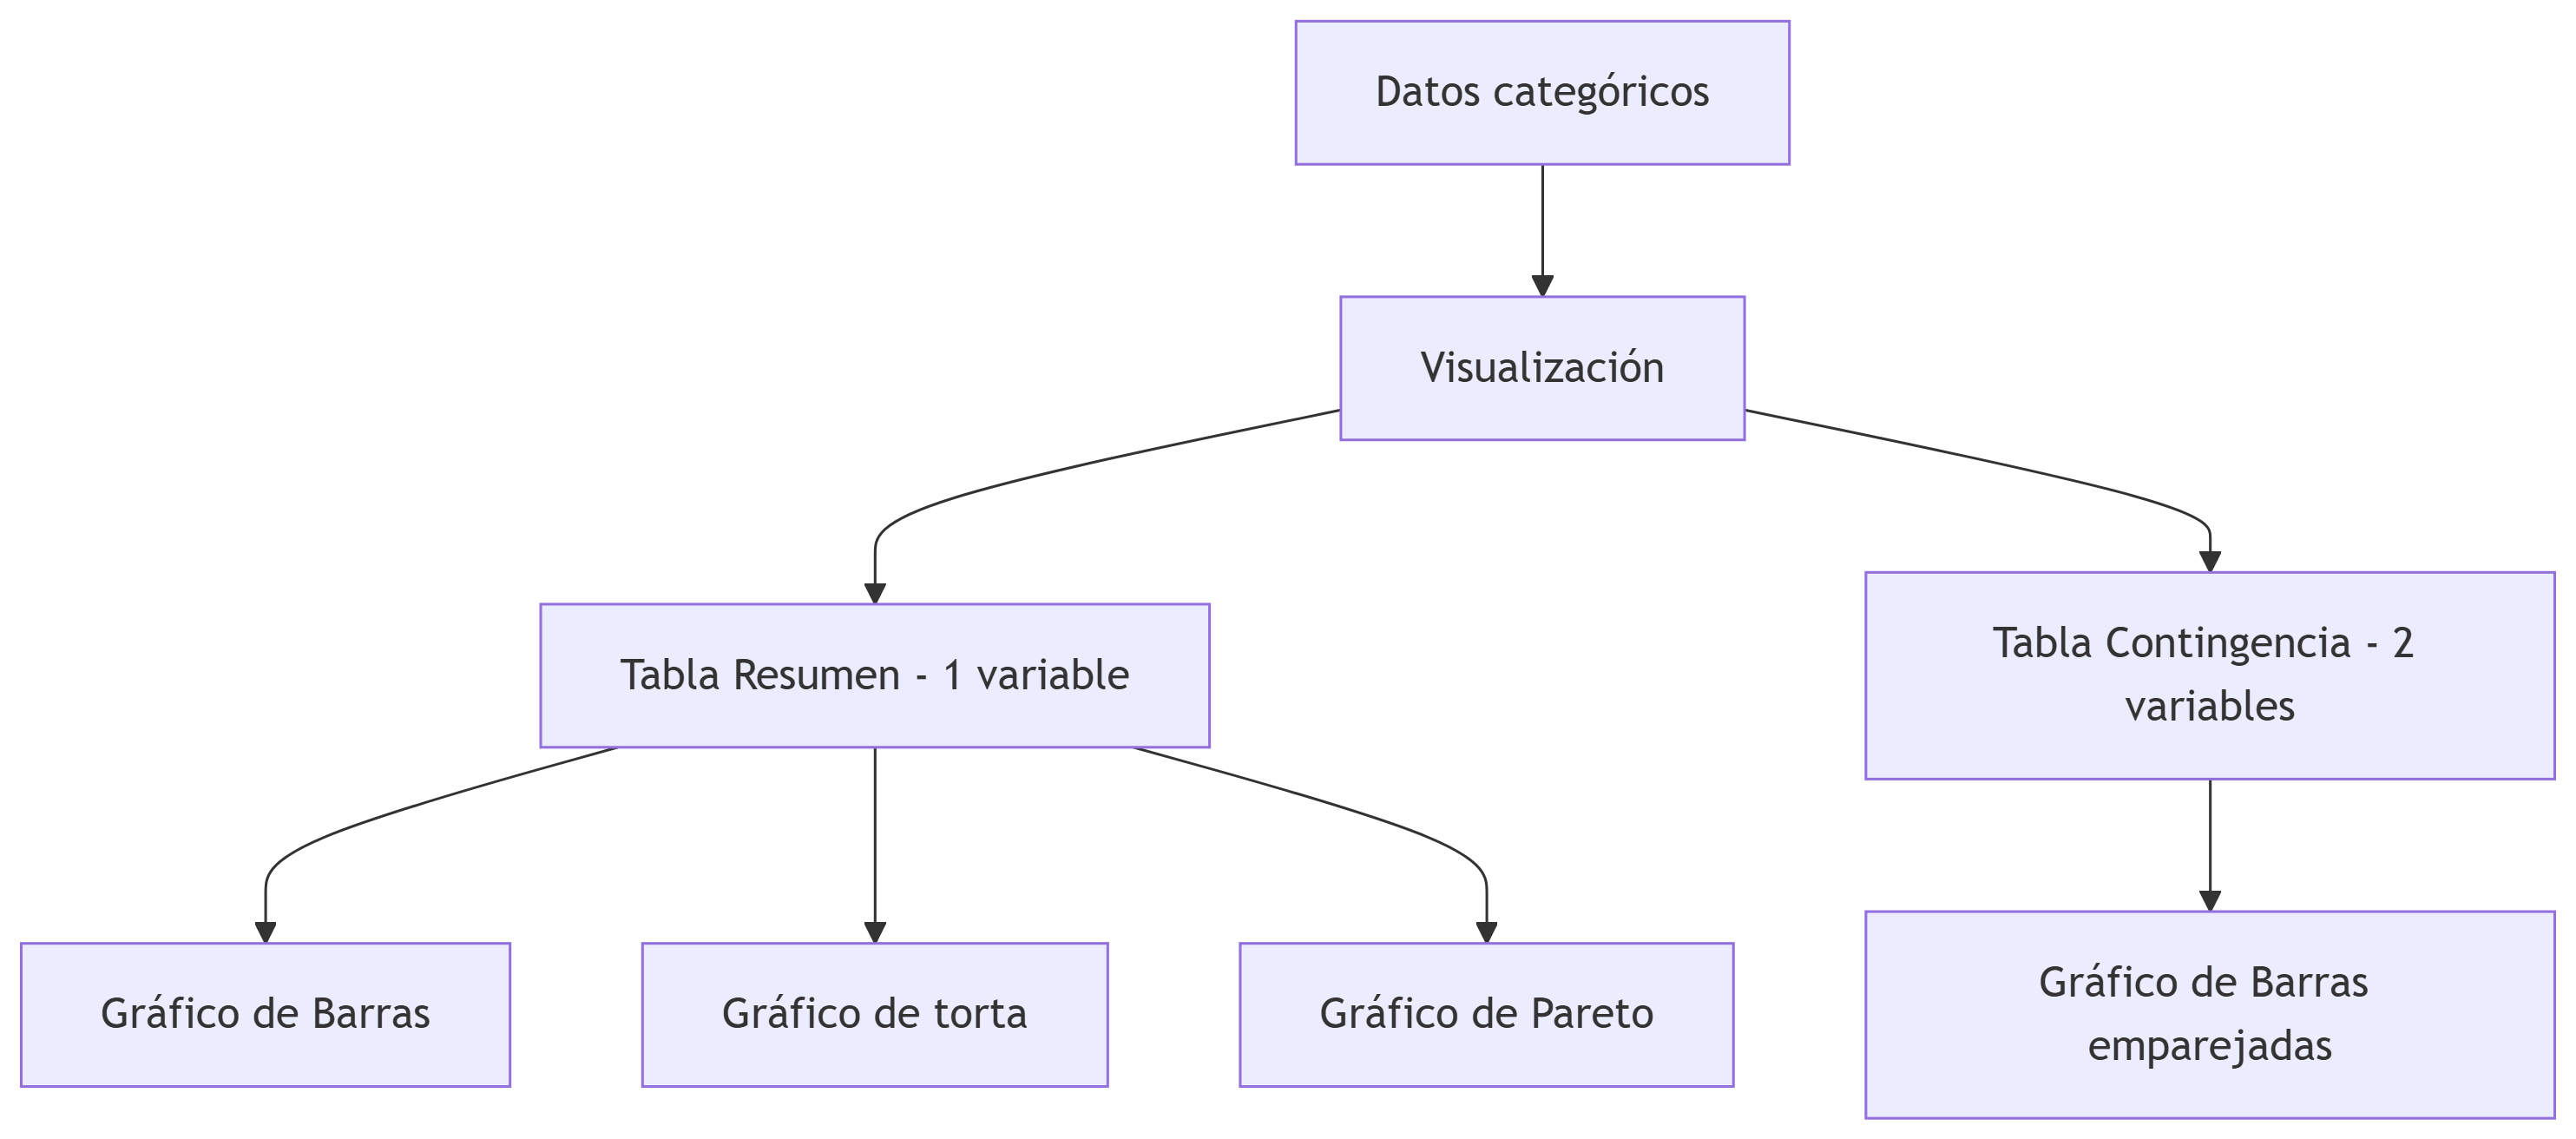
\includegraphics[width=10.13in,height=4.48in]{capitulo2_files/figure-latex/mermaid-figure-2.png}

Opciones de Visualización para Datos Categóricos

\subsection{Visualizando datos
numéricos}\label{visualizando-datos-numuxe9ricos}

\subsubsection{Distribución de
frecuencia}\label{distribuciuxf3n-de-frecuencia}

Imagina que registras el \textbf{monto gastado por cada cliente} en tu
restaurante durante un día. Tienes muchos valores sueltos y quieres
resumirlos para entender mejor los patrones.

La \textbf{distribución de frecuencia} es una tabla que agrupa esos
montos en \textbf{categorías numéricas ordenadas} (también llamadas
clases) y cuenta cuántos clientes caen en cada una.

\textbf{¿Cómo elegir las categorías?}

Primero necesitas definir \textbf{categorías adecuadas}: decidir sus
límites (fronteras) y su \textbf{ancho}.\\
El número de categorías depende del \textbf{rango} de los datos (máximo
-- mínimo). Si los gastos van desde \$5 hasta \$55, el rango es 50.\\
Cuando el rango es grande solemos usar más categorías; en la práctica,
entre \textbf{5 y 15} funciona bien.

\textbf{¿Cómo calcular el ancho?}

Si decides usar, por ejemplo, 10 categorías:

\[
\text{Ancho} = \frac{\text{Rango}}{\text{Número de categorías}} = \frac{50}{10} = 5
\]

Eso significa que tus clases podrían ser: \$5--\textless\$10,
\$10--\textless\$15, \$15--\textless\$20, \ldots{} hasta \$55. Luego
cuentas cuántos clientes gastaron en cada intervalo y obtienes una tabla
clara para analizar tendencias (por ejemplo, ``la mayoría gasta entre
\$15 y \$25'').

Esta tabla te permite pasar del desorden de datos individuales a una
visión estructurada que facilita la toma de decisiones.

\textbf{Ejemplo práctico: Distribución de gastos}

Supongamos que registramos el gasto de \textbf{100 clientes} y los
agrupamos usando intervalos de \$5:

\begin{longtable}[]{@{}
  >{\centering\arraybackslash}p{(\linewidth - 8\tabcolsep) * \real{0.2394}}
  >{\centering\arraybackslash}p{(\linewidth - 8\tabcolsep) * \real{0.1690}}
  >{\centering\arraybackslash}p{(\linewidth - 8\tabcolsep) * \real{0.1690}}
  >{\centering\arraybackslash}p{(\linewidth - 8\tabcolsep) * \real{0.2394}}
  >{\centering\arraybackslash}p{(\linewidth - 8\tabcolsep) * \real{0.1831}}@{}}
\caption{Distribución de Gastos por
Cliente}\label{tbl-distribucion-gastos}\tabularnewline
\toprule\noalign{}
\begin{minipage}[b]{\linewidth}\centering
Intervalo (USD)
\end{minipage} & \begin{minipage}[b]{\linewidth}\centering
Frecuencia
\end{minipage} & \begin{minipage}[b]{\linewidth}\centering
\% Relativo
\end{minipage} & \begin{minipage}[b]{\linewidth}\centering
Frec. Acumulada
\end{minipage} & \begin{minipage}[b]{\linewidth}\centering
\% Acumulado
\end{minipage} \\
\midrule\noalign{}
\endfirsthead
\toprule\noalign{}
\begin{minipage}[b]{\linewidth}\centering
Intervalo (USD)
\end{minipage} & \begin{minipage}[b]{\linewidth}\centering
Frecuencia
\end{minipage} & \begin{minipage}[b]{\linewidth}\centering
\% Relativo
\end{minipage} & \begin{minipage}[b]{\linewidth}\centering
Frec. Acumulada
\end{minipage} & \begin{minipage}[b]{\linewidth}\centering
\% Acumulado
\end{minipage} \\
\midrule\noalign{}
\endhead
\bottomrule\noalign{}
\endlastfoot
\$5 - \textless\$10 & 8 & 8\% & 8 & 8\% \\
\$10 - \textless\$15 & 15 & 15\% & 23 & 23\% \\
\$15 - \textless\$20 & 22 & 22\% & 45 & 45\% \\
\$20 - \textless\$25 & 25 & 25\% & 70 & 70\% \\
\$25 - \textless\$30 & 14 & 14\% & 84 & 84\% \\
\$30 - \textless\$35 & 9 & 9\% & 93 & 93\% \\
\$35 - \textless\$40 & 5 & 5\% & 98 & 98\% \\
\$40 - \textless\$45 & 2 & 2\% & 100 & 100\% \\
\textbf{Total} & \textbf{100} & \textbf{100\%} & - & - \\
\end{longtable}

\textbf{Interpretación clave:}

\begin{itemize}
\tightlist
\item
  \textbf{Concentración:} El 70\% de los clientes gastó menos de \$25
\item
  \textbf{Cola:} Solo el 7\% gastó más de \$35
\item
  \textbf{Patrón:} La mayoría de clientes (67\%) gasta entre \$10-\$30
\end{itemize}

\subsubsection{Histograma}\label{histograma}

Siguiendo con el ejemplo de los gastos en el restaurante, el
\textbf{histograma} es la versión gráfica de la tabla de distribución de
frecuencia.\\
En lugar de mostrar los números en una tabla, dibujamos una barra para
cada categoría (intervalo de gasto).

\begin{itemize}
\tightlist
\item
  El \textbf{eje horizontal} muestra los intervalos: \$5--\textless\$10,
  \$10--\textless\$15, etc.\\
\item
  El \textbf{eje vertical} muestra la frecuencia (o el porcentaje) de
  clientes en cada intervalo.\\
\item
  Las barras van \textbf{pegadas} porque los intervalos son continuos:
  representan rangos de una misma variable numérica.
\end{itemize}

\begin{figure}

\centering{

\pandocbounded{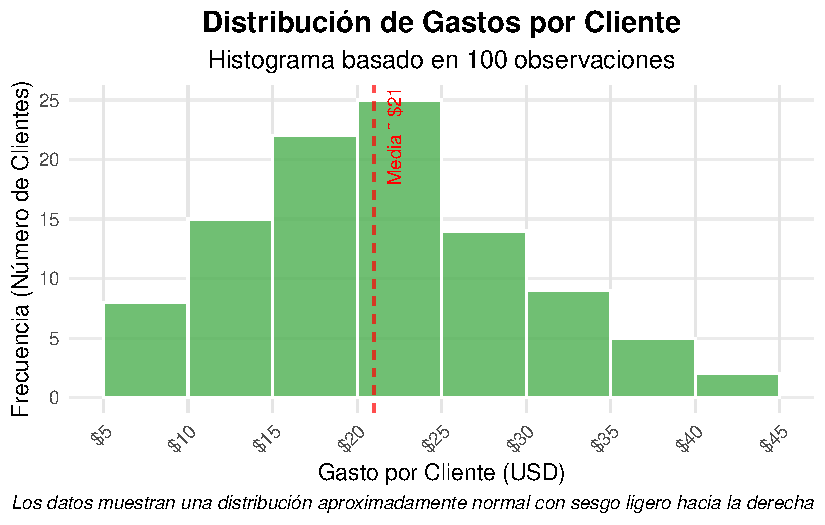
\includegraphics[keepaspectratio]{capitulo2_files/figure-pdf/fig-histograma-gastos-1.pdf}}

}

\caption{\label{fig-histograma-gastos}Histograma - Distribución de
Gastos por Cliente}

\end{figure}%

Un \textbf{histograma} es la representación gráfica de una distribución
de frecuencias para datos numéricos continuos. A diferencia del gráfico
de barras (para datos categóricos), el histograma muestra barras
adyacentes sin espacios entre ellas, lo que refleja la naturaleza
continua de los datos.

\textbf{Características clave del histograma:}

\begin{itemize}
\tightlist
\item
  \textbf{Eje X:} Intervalos de valores (clases) de la variable numérica
\item
  \textbf{Eje Y:} Frecuencia (cantidad de observaciones en cada
  intervalo)
\item
  \textbf{Barras conectadas:} Sin espacios, indicando continuidad de los
  datos
\item
  \textbf{Forma de distribución:} Permite identificar patrones como
  simetría, sesgo o multimodalidad
\end{itemize}

El histograma nos permite visualizar rápidamente:

\begin{itemize}
\tightlist
\item
  \textbf{¿Dónde se concentran los datos?} (moda o pico más alto)
\item
  \textbf{¿Cómo se distribuyen?} (simétrica, sesgada a la
  izquierda/derecha)
\item
  \textbf{¿Hay valores atípicos?} (barras aisladas en los extremos)
\end{itemize}

\begin{tcolorbox}[enhanced jigsaw, arc=.35mm, leftrule=.75mm, colbacktitle=quarto-callout-note-color!10!white, left=2mm, opacitybacktitle=0.6, toptitle=1mm, title=\textcolor{quarto-callout-note-color}{\faInfo}\hspace{0.5em}{Interpretación del histograma}, colframe=quarto-callout-note-color-frame, toprule=.15mm, colback=white, rightrule=.15mm, opacityback=0, coltitle=black, breakable, bottomtitle=1mm, titlerule=0mm, bottomrule=.15mm]

\textbf{Forma de la distribución:}

\begin{itemize}
\tightlist
\item
  \textbf{Aproximadamente normal:} La distribución tiene forma de
  campana con un pico central
\item
  \textbf{Sesgo ligero:} Hay una ``cola'' más larga hacia la derecha
  (valores altos)
\item
  \textbf{Concentración:} La mayoría de clientes gasta entre \$15-\$30
\end{itemize}

\textbf{Información práctica:}

\begin{itemize}
\tightlist
\item
  \textbf{Valor típico:} Alrededor de \$20-\$25 (pico del histograma)
\item
  \textbf{Rango común:} El 70\% de clientes gasta menos de \$25
\item
  \textbf{Valores extremos:} Muy pocos clientes gastan más de \$35
\end{itemize}

\end{tcolorbox}

\textbf{¿Cuándo usar un histograma vs.~gráfico de barras?}

\begin{longtable}[]{@{}
  >{\raggedright\arraybackslash}p{(\linewidth - 4\tabcolsep) * \real{0.2439}}
  >{\raggedright\arraybackslash}p{(\linewidth - 4\tabcolsep) * \real{0.2927}}
  >{\raggedright\arraybackslash}p{(\linewidth - 4\tabcolsep) * \real{0.4634}}@{}}
\caption{Histograma vs.~Gráfico de
Barras}\label{tbl-histograma-vs-barras}\tabularnewline
\toprule\noalign{}
\begin{minipage}[b]{\linewidth}\raggedright
Criterio
\end{minipage} & \begin{minipage}[b]{\linewidth}\raggedright
Histograma
\end{minipage} & \begin{minipage}[b]{\linewidth}\raggedright
Gráfico de Barras
\end{minipage} \\
\midrule\noalign{}
\endfirsthead
\toprule\noalign{}
\begin{minipage}[b]{\linewidth}\raggedright
Criterio
\end{minipage} & \begin{minipage}[b]{\linewidth}\raggedright
Histograma
\end{minipage} & \begin{minipage}[b]{\linewidth}\raggedright
Gráfico de Barras
\end{minipage} \\
\midrule\noalign{}
\endhead
\bottomrule\noalign{}
\endlastfoot
\textbf{Tipo de datos} & Numéricos continuos & Categóricos \\
\textbf{Separación de barras} & Sin espacios (datos continuos) & Con
espacios (categorías distintas) \\
\textbf{Objetivo principal} & Mostrar distribución de frecuencias &
Comparar categorías \\
\textbf{Ejemplo} & Edades, pesos, tiempos & Colores, marcas, géneros \\
\end{longtable}

\subsubsection{Gráfico de Dispersión}\label{gruxe1fico-de-dispersiuxf3n}

El \textbf{gráfico de dispersión} (scatter plot) es la herramienta
principal para visualizar la \textbf{relación entre dos variables
numéricas}. A diferencia del histograma que muestra una sola variable,
el gráfico de dispersión permite explorar si existe algún patrón,
tendencia o correlación entre dos mediciones diferentes.

Sigamos con el restaurante: además del \textbf{gasto de cada cliente}
(en dólares), registramos el \textbf{tiempo que permanecen} en el
establecimiento (en minutos). Queremos saber si existe alguna relación
entre estas dos variables continuas.

En el gráfico de dispersión: - Cada \textbf{punto} representa a un
cliente individual. - El \textbf{eje X} muestra el tiempo de permanencia
(en minutos). - El \textbf{eje Y} muestra el gasto total de ese cliente
(en dólares).

\textbf{Patrones que puedes identificar:}

\begin{tcolorbox}[enhanced jigsaw, arc=.35mm, leftrule=.75mm, colbacktitle=quarto-callout-tip-color!10!white, left=2mm, opacitybacktitle=0.6, toptitle=1mm, title=\textcolor{quarto-callout-tip-color}{\faLightbulb}\hspace{0.5em}{Tipos de relaciones en un gráfico de dispersión}, colframe=quarto-callout-tip-color-frame, toprule=.15mm, colback=white, rightrule=.15mm, opacityback=0, coltitle=black, breakable, bottomtitle=1mm, titlerule=0mm, bottomrule=.15mm]

\begin{itemize}
\tightlist
\item
  \textbf{Correlación positiva:} Los puntos forman una nube que asciende
  (↗). A mayor X, mayor Y
\item
  \textbf{Correlación negativa:} Los puntos forman una nube que
  desciende (↘). A mayor X, menor Y\\
\item
  \textbf{Sin correlación:} Los puntos se distribuyen aleatoriamente sin
  patrón claro
\item
  \textbf{Correlación curvilínea:} Los puntos siguen una curva (ej.
  forma de U o parábola)
\end{itemize}

\end{tcolorbox}

\begin{figure}

\centering{

\pandocbounded{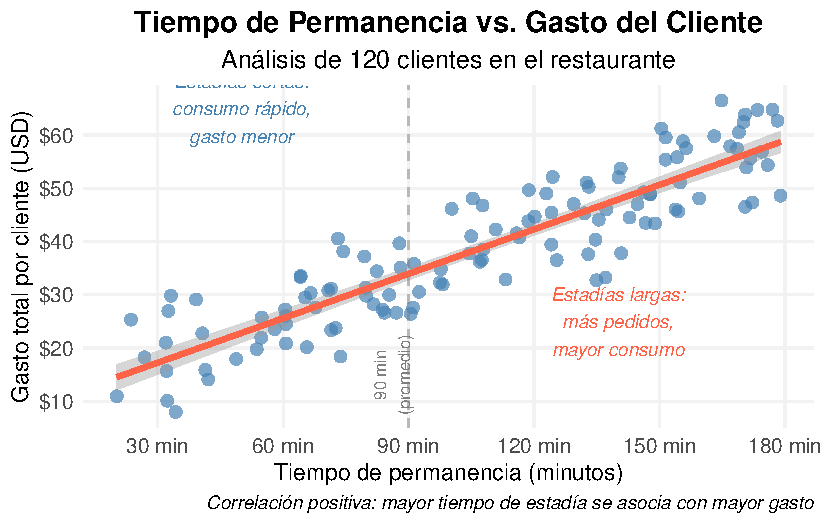
\includegraphics[keepaspectratio]{capitulo2_files/figure-pdf/fig-dispersion-tiempo-gasto-1.pdf}}

}

\caption{\label{fig-dispersion-tiempo-gasto}Gráfico de Dispersión -
Relación entre Tiempo de Permanencia y Gasto del Cliente}

\end{figure}%

\textbf{Interpretación del gráfico de dispersión:}

El ejemplo muestra una \textbf{correlación positiva} entre el tiempo de
permanencia y el gasto del cliente. Esta relación tiene sentido desde la
perspectiva del negocio:

\begin{itemize}
\tightlist
\item
  \textbf{Tendencia ascendente:} Los clientes que permanecen más tiempo
  tienden a gastar más
\item
  \textbf{Relación lógica:} Más tiempo permite más pedidos (aperitivos,
  postres, bebidas adicionales)
\item
  \textbf{Variabilidad natural:} No todos los puntos siguen la línea
  perfectamente - algunos clientes gastan mucho en poco tiempo (pedidos
  caros) y otros gastan poco aunque permanezcan mucho tiempo
\item
  \textbf{Rango de comportamientos:} Clientes con estadías cortas (20-60
  min) gastan típicamente \$8-\$30, mientras que los de estadías largas
  (120-180 min) gastan frecuentemente \$35-\$70
\end{itemize}

\textbf{Insights para el negocio:}

\begin{itemize}
\tightlist
\item
  \textbf{Estrategia de retención:} Mantener a los clientes más tiempo
  puede \textbf{incrementar las ventas}
\item
  \textbf{Ambiente acogedor:} Espacios cómodos que inviten a quedarse
  más tiempo
\item
  \textbf{Menú estratégico:} Ofrecer aperitivos, postres y bebidas para
  \textbf{extender la experiencia}
\item
  \textbf{Identificar oportunidades:} Clientes con estadías largas pero
  bajo gasto podrían necesitar más atención del mesero
\end{itemize}

\begin{tcolorbox}[enhanced jigsaw, arc=.35mm, leftrule=.75mm, colbacktitle=quarto-callout-note-color!10!white, left=2mm, opacitybacktitle=0.6, toptitle=1mm, title=\textcolor{quarto-callout-note-color}{\faInfo}\hspace{0.5em}{¿Cuándo usar un gráfico de dispersión?}, colframe=quarto-callout-note-color-frame, toprule=.15mm, colback=white, rightrule=.15mm, opacityback=0, coltitle=black, breakable, bottomtitle=1mm, titlerule=0mm, bottomrule=.15mm]

\textbf{Ideal para:}

\begin{itemize}
\tightlist
\item
  Explorar relaciones entre dos variables numéricas
\item
  Identificar correlaciones positivas, negativas o ausencia de
  correlación\\
\item
  Detectar valores atípicos (outliers)
\item
  Validar supuestos antes de análisis estadísticos más avanzados
\end{itemize}

\textbf{Limitaciones:}

\begin{itemize}
\tightlist
\item
  Solo muestra dos variables a la vez
\item
  La correlación no implica causalidad
\item
  Puede ser difícil interpretar con muchos puntos sobrepuestos
\end{itemize}

\end{tcolorbox}

\bookmarksetup{startatroot}

\chapter{Explorando tus Datos con Estadísticos
Descriptivos}\label{explorando-tus-datos-con-estaduxedsticos-descriptivos}

Imagina que eres gerente de un restaurante que acaba de lanzar un nuevo
menú y quieres evaluar la satisfacción de tus clientes a partir de las
calificaciones que te han dado. Tienes cientos de puntuaciones y
necesitas entender rápidamente cuál es la opinión general, qué tan
variadas son las experiencias y si hay patrones o valores atípicos que
merecen atención.

¿Cómo puedes resumir y comprender toda esa información de forma clara y
sencilla? Para eso utilizamos los estadísticos descriptivos,
herramientas fundamentales que nos permiten condensar grandes cantidades
de datos en medidas simples y significativas.

Estas medidas serán esenciales para tomar decisiones informadas que
mejoren tu decisiones.

\section{Estadísticos Descriptivos}\label{estaduxedsticos-descriptivos}

Los estadísticos descriptivos son herramientas clave que nos permiten
resumir y comprender mejor la información contenida en nuestros datos.
Para facilitar su estudio, los podemos clasificar en cuatro categorías
principales:

\begin{itemize}
\tightlist
\item
  \textbf{Medidas de tendencia central}: Estas nos muestran el valor
  típico o representativo en un conjunto de datos, es decir, alrededor
  de qué número se agrupan la mayoría de las observaciones.
\item
  \textbf{Medidas de variación}: Nos indican qué tan dispersos o
  concentrados están los datos respecto a esa tendencia central,
  ayudándonos a entender la consistencia o diversidad dentro de la
  información.
\item
  \textbf{Medidas de forma}: Describen la distribución general de los
  datos, revelando si están simétricos, sesgados hacia un lado o
  presentan picos o colas particulares.
\item
  \textbf{Medidas de relación}: Evalúan cómo dos variables numéricas se
  relacionan entre sí, especialmente si existe una conexión lineal que
  pueda ser útil para análisis más avanzados.
\end{itemize}

\section{Medidas de Tendencia
Central}\label{medidas-de-tendencia-central}

Cuando queremos entender las calificaciones que los clientes dan a tu
restaurante, buscamos encontrar un valor que represente lo que la
mayoría piensa. Las medidas de tendencia central nos ayudan a esto.

\subsection{Media (Promedio)}\label{media-promedio}

La media o promedio es una forma simple pero útil de resumir un conjunto
de datos. La media es el valor que obtienes al sumar todas las
calificaciones y dividirlas entre el número total de clientes.

\begin{tcolorbox}[enhanced jigsaw, arc=.35mm, leftrule=.75mm, opacityback=0, left=2mm, breakable, colframe=quarto-callout-tip-color-frame, toprule=.15mm, colback=white, bottomrule=.15mm, rightrule=.15mm]
\begin{minipage}[t]{5.5mm}
\textcolor{quarto-callout-tip-color}{\faLightbulb}
\end{minipage}%
\begin{minipage}[t]{\textwidth - 5.5mm}

Matemáticamente se escribiría así:

\[
\text{Media} = \bar{x} = \frac{x_1 + x_2 + \cdots + x_n}{n}
\]

\end{minipage}%
\end{tcolorbox}

Por ejemplo, si cinco clientes dieron las calificaciones: 4, 5, 3, 4 y
5, la media será:

\begin{tcolorbox}[enhanced jigsaw, arc=.35mm, leftrule=.75mm, opacityback=0, left=2mm, breakable, colframe=quarto-callout-tip-color-frame, toprule=.15mm, colback=white, bottomrule=.15mm, rightrule=.15mm]
\begin{minipage}[t]{5.5mm}
\textcolor{quarto-callout-tip-color}{\faLightbulb}
\end{minipage}%
\begin{minipage}[t]{\textwidth - 5.5mm}

\[
\bar{x} = \frac{4 + 5 + 3 + 4 + 5}{5} = \frac{21}{5} = 4.2
\]

\end{minipage}%
\end{tcolorbox}

Sin embargo la media, tiene limitaciones: no muestra cómo están
distribuidos los datos y puede ser engañosa si hay grandes diferencias
entre los valores. Por ejemplo:

\begin{center}
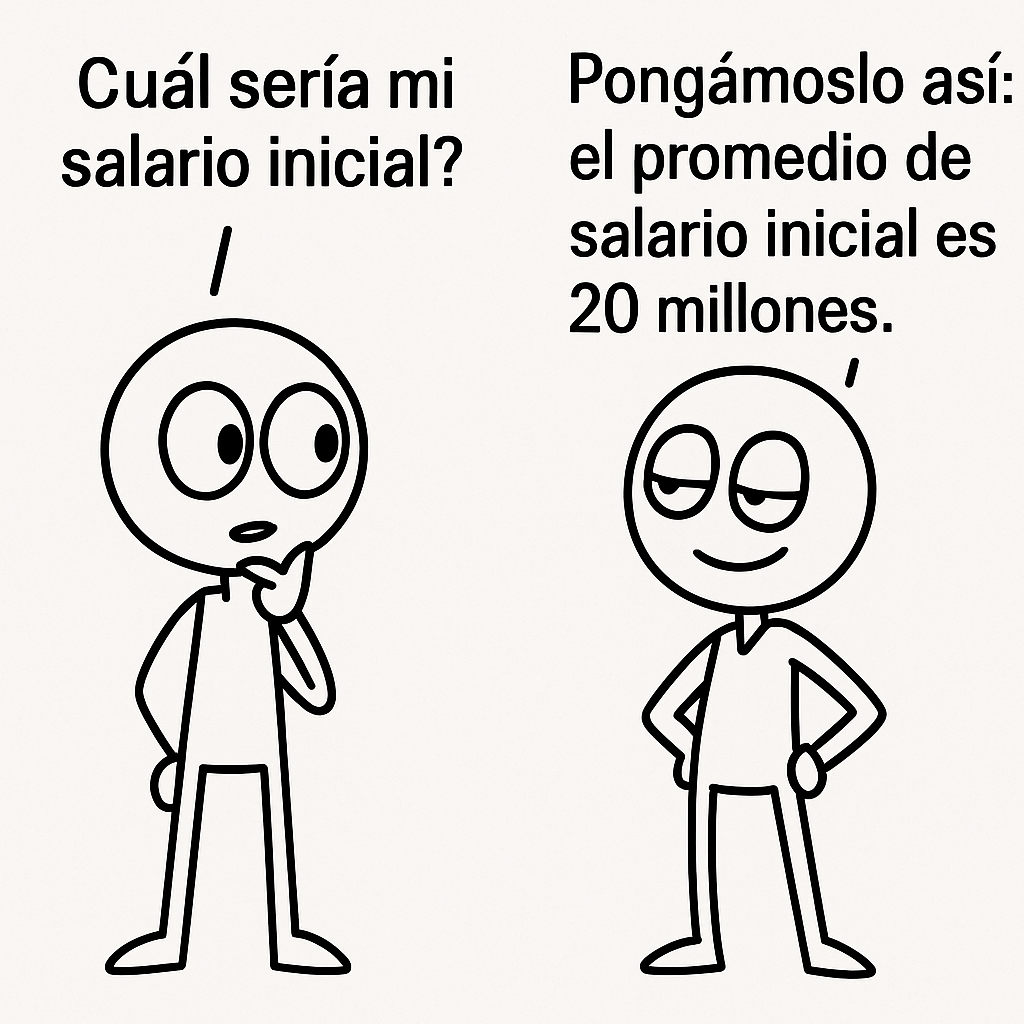
\includegraphics[width=3.64583in,height=\textheight,keepaspectratio]{img/media_1.png}
\end{center}

\begin{center}
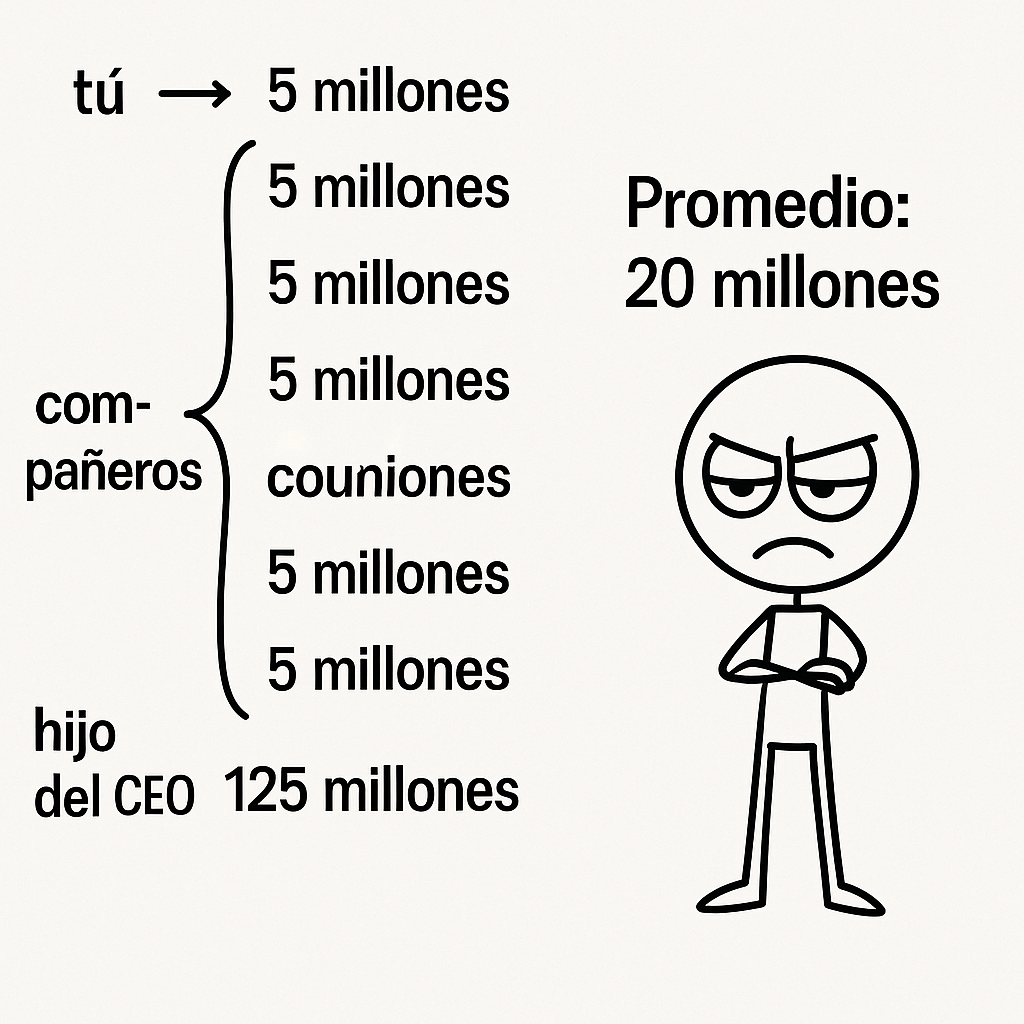
\includegraphics[width=3.64583in,height=\textheight,keepaspectratio]{img/media_2.png}
\end{center}

Aquí hay otro ejemplo donde la media es la misma en ambas situaciones
pero el contexto individual que esconde es muy diferente:

\begin{center}
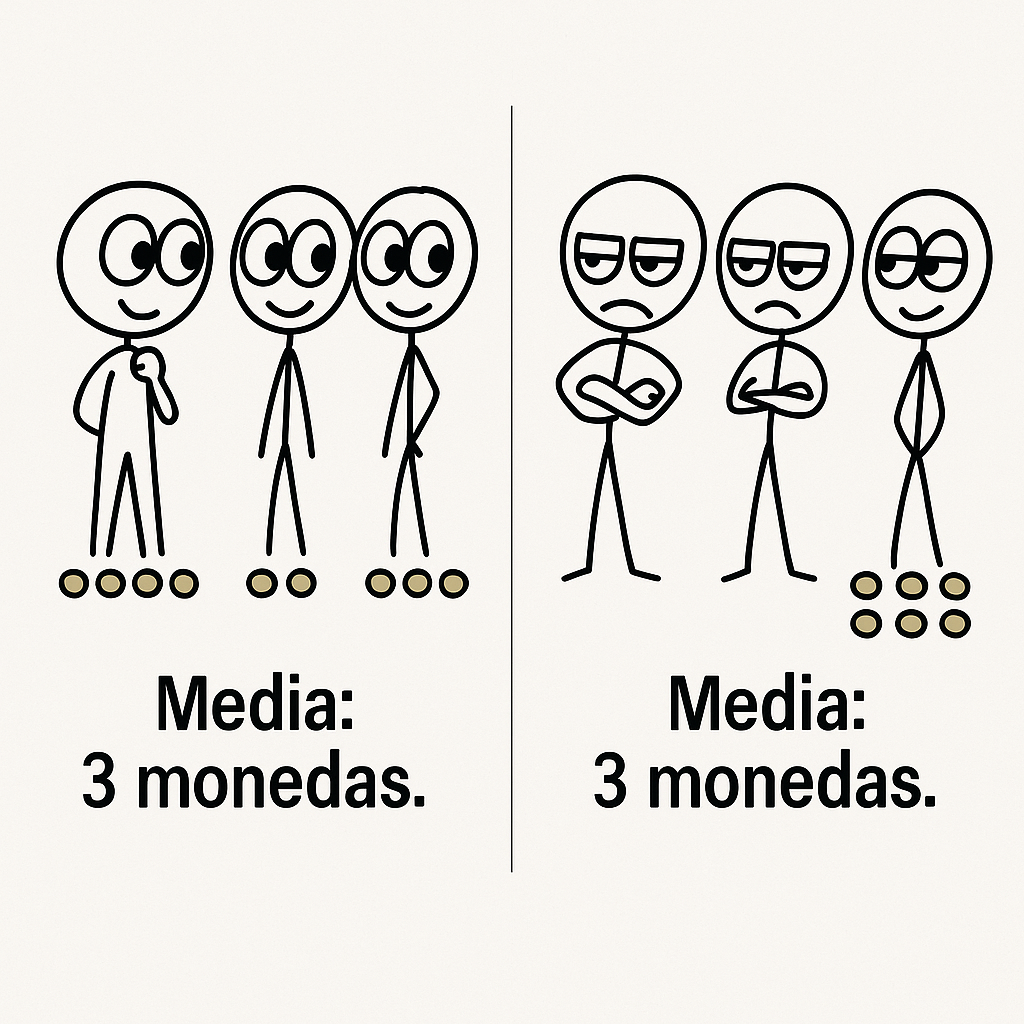
\includegraphics[width=3.64583in,height=\textheight,keepaspectratio]{img/media_3.png}
\end{center}

\subsection{Mediana}\label{mediana}

Volviendo a las calificaciones de tu restaurante, la \textbf{mediana} es
el valor que está justo en el medio cuando ordenas todas las opiniones
de menor a mayor. Esto significa que la mitad de los clientes dieron una
calificación igual o menor que la mediana, y la otra mitad dio una
calificación igual o mayor.

Por ejemplo, si tus clientes calificaron así: 3, 4, 4, 5, 5, la mediana
es 4 --- porque es el valor que divide el grupo en dos partes iguales.

\begin{tcolorbox}[enhanced jigsaw, arc=.35mm, leftrule=.75mm, opacityback=0, left=2mm, breakable, colframe=quarto-callout-tip-color-frame, toprule=.15mm, colback=white, bottomrule=.15mm, rightrule=.15mm]
\begin{minipage}[t]{5.5mm}
\textcolor{quarto-callout-tip-color}{\faLightbulb}
\end{minipage}%
\begin{minipage}[t]{\textwidth - 5.5mm}

\[
\text{Mediana} = \text{valor central en datos ordenados}
\]

\end{minipage}%
\end{tcolorbox}

Una gran ventaja de la mediana es que \textbf{no se ve afectada por
calificaciones muy bajas o muy altas} que podrían distorsionar la media.
Por ejemplo, si alguien puso un 1 o un 10, la mediana sigue mostrando el
punto medio real de la mayoría.

Sin embargo, la mediana \textbf{no nos dice qué tan dispersas están las
calificaciones a cada lado}. Por eso, para entender mejor la
variabilidad de las opiniones, necesitaremos otras medidas que veremos
más adelante.

A continuación podemos ver un ejemplo donde la mediana es usada para
entregar un mensaje erróneo:

\begin{center}
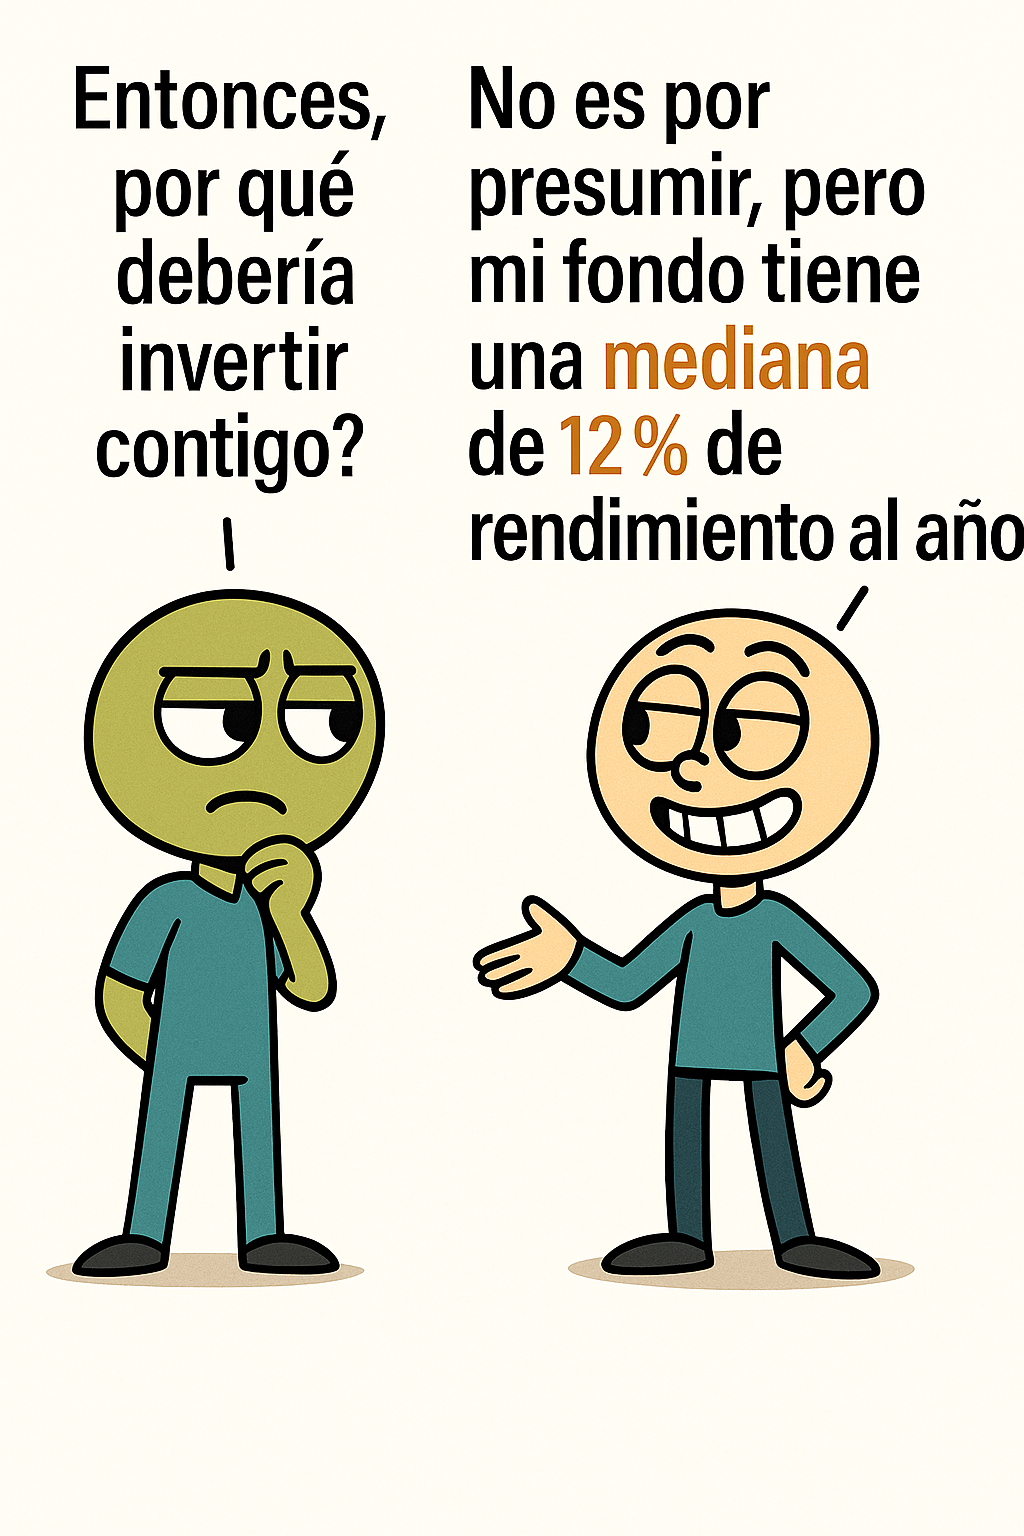
\includegraphics[width=3.64583in,height=\textheight,keepaspectratio]{img/mediana_1.png}
\end{center}

Pero, los rendimientos anuales del fondo:

\begin{center}
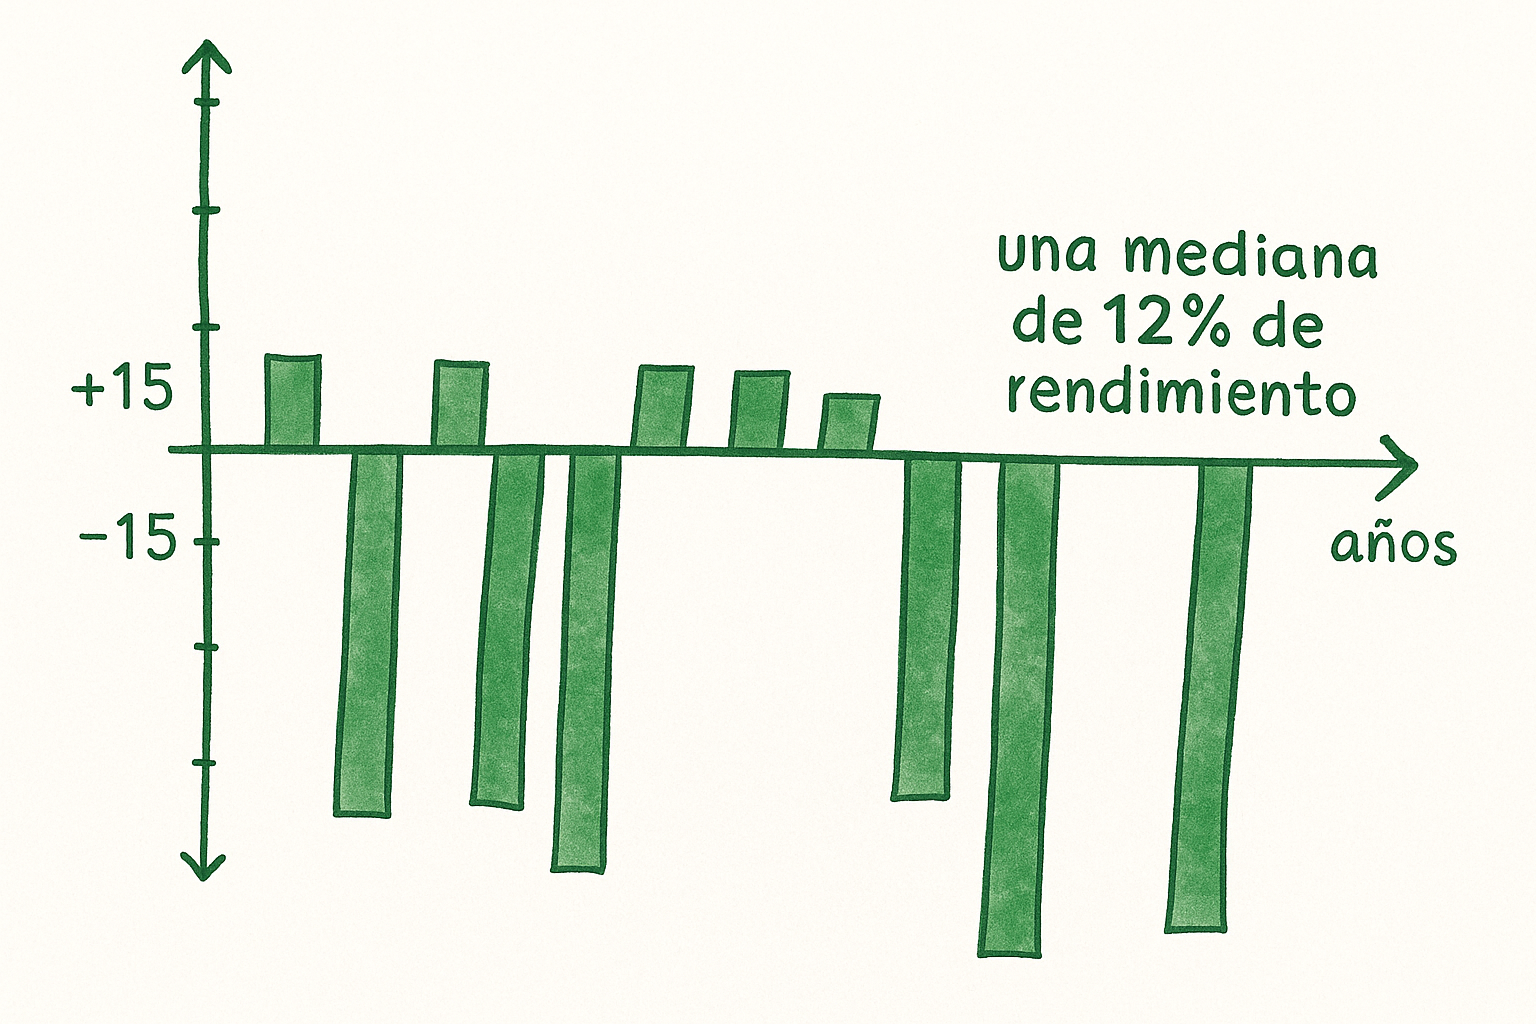
\includegraphics[width=3.64583in,height=\textheight,keepaspectratio]{img/mediana_2.png}
\end{center}

Miremos otro ejemplo donde la mediana similar no implica datos
similares. Siempre hay tener una combinación de datos para tomar
decisiones correctas

\begin{center}
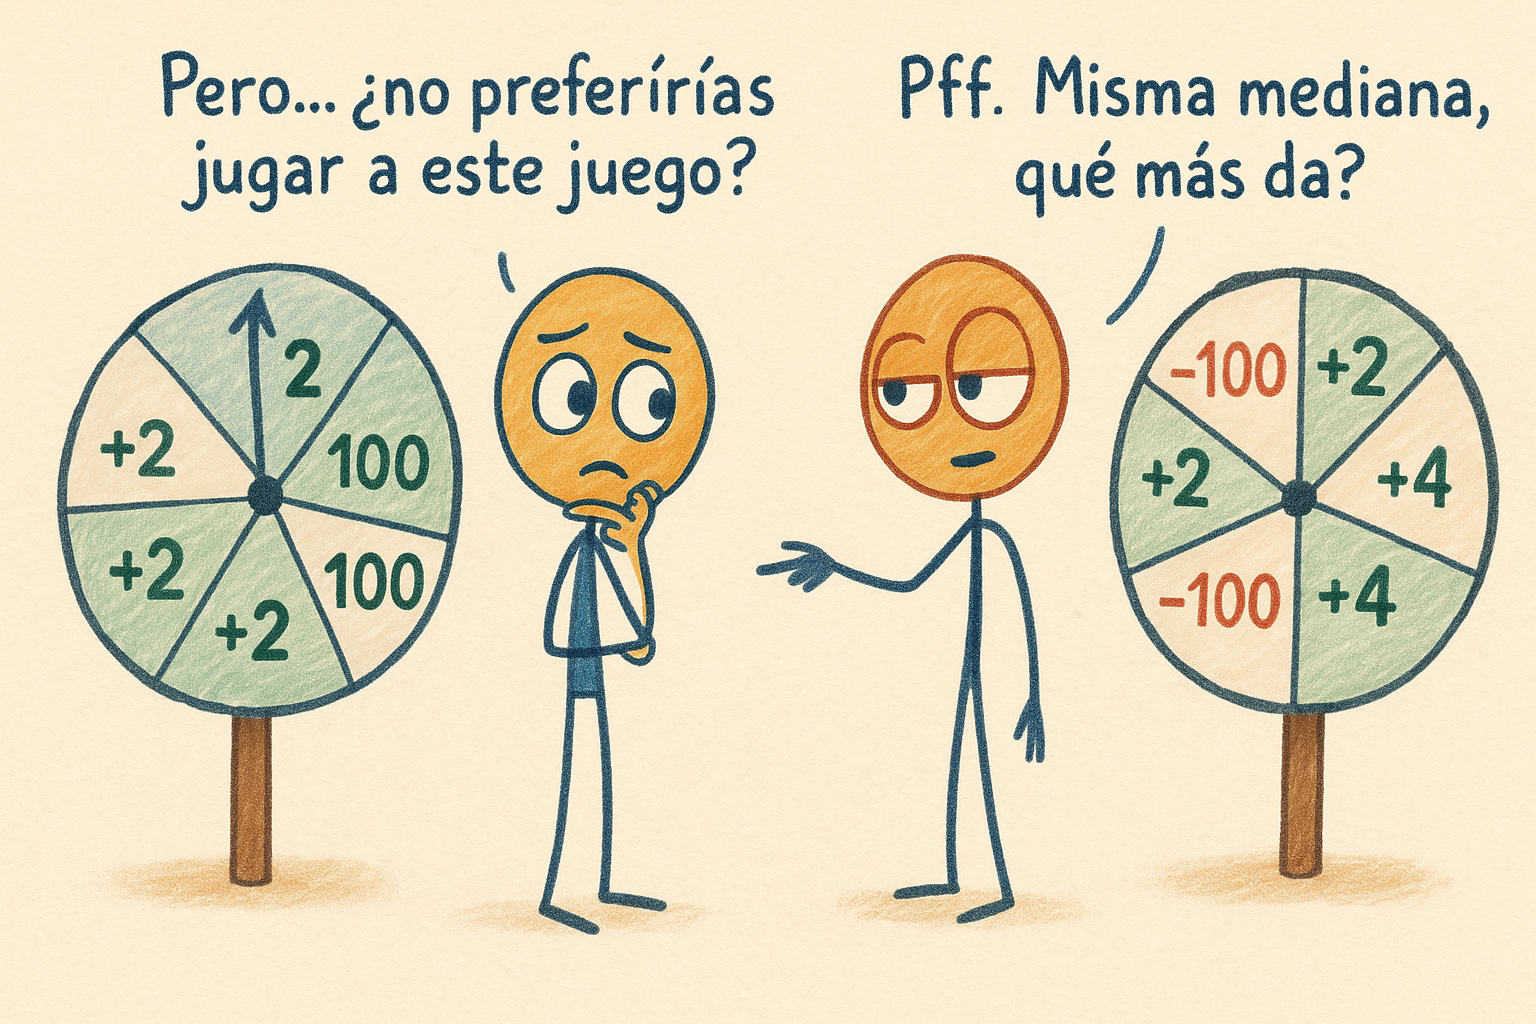
\includegraphics[width=3.64583in,height=\textheight,keepaspectratio]{img/mediana_3.png}
\end{center}

\subsection{Moda}\label{moda}

La \textbf{moda} es la calificación que más se repite entre tus
clientes. Es como la opinión más común o popular sobre tu restaurante.

Por ejemplo, si las calificaciones de tus clientes fueron: 3, 4, 4, 5,
5, tanto 4 como 5 se repiten dos veces, por lo que hay dos modas: 4 y 5.

Si no hay repeticiones exactas, se pueden agrupar en categorías y tomar
como moda la más común. Es útil especialmente con datos no numéricos,
como colores o preferencias políticas, donde no tiene sentido calcular
promedios.

\begin{tcolorbox}[enhanced jigsaw, arc=.35mm, leftrule=.75mm, opacityback=0, left=2mm, breakable, colframe=quarto-callout-tip-color-frame, toprule=.15mm, colback=white, bottomrule=.15mm, rightrule=.15mm]
\begin{minipage}[t]{5.5mm}
\textcolor{quarto-callout-tip-color}{\faLightbulb}
\end{minipage}%
\begin{minipage}[t]{\textwidth - 5.5mm}

\[
\text{Moda} = \text{valor que aparece con mayor frecuencia}
\]

\end{minipage}%
\end{tcolorbox}

Su limitación: no considera la totalidad ni la distribución de los
datos, y lo más común no siempre es lo más representativo. Miremos este
ejemplo:

\begin{center}
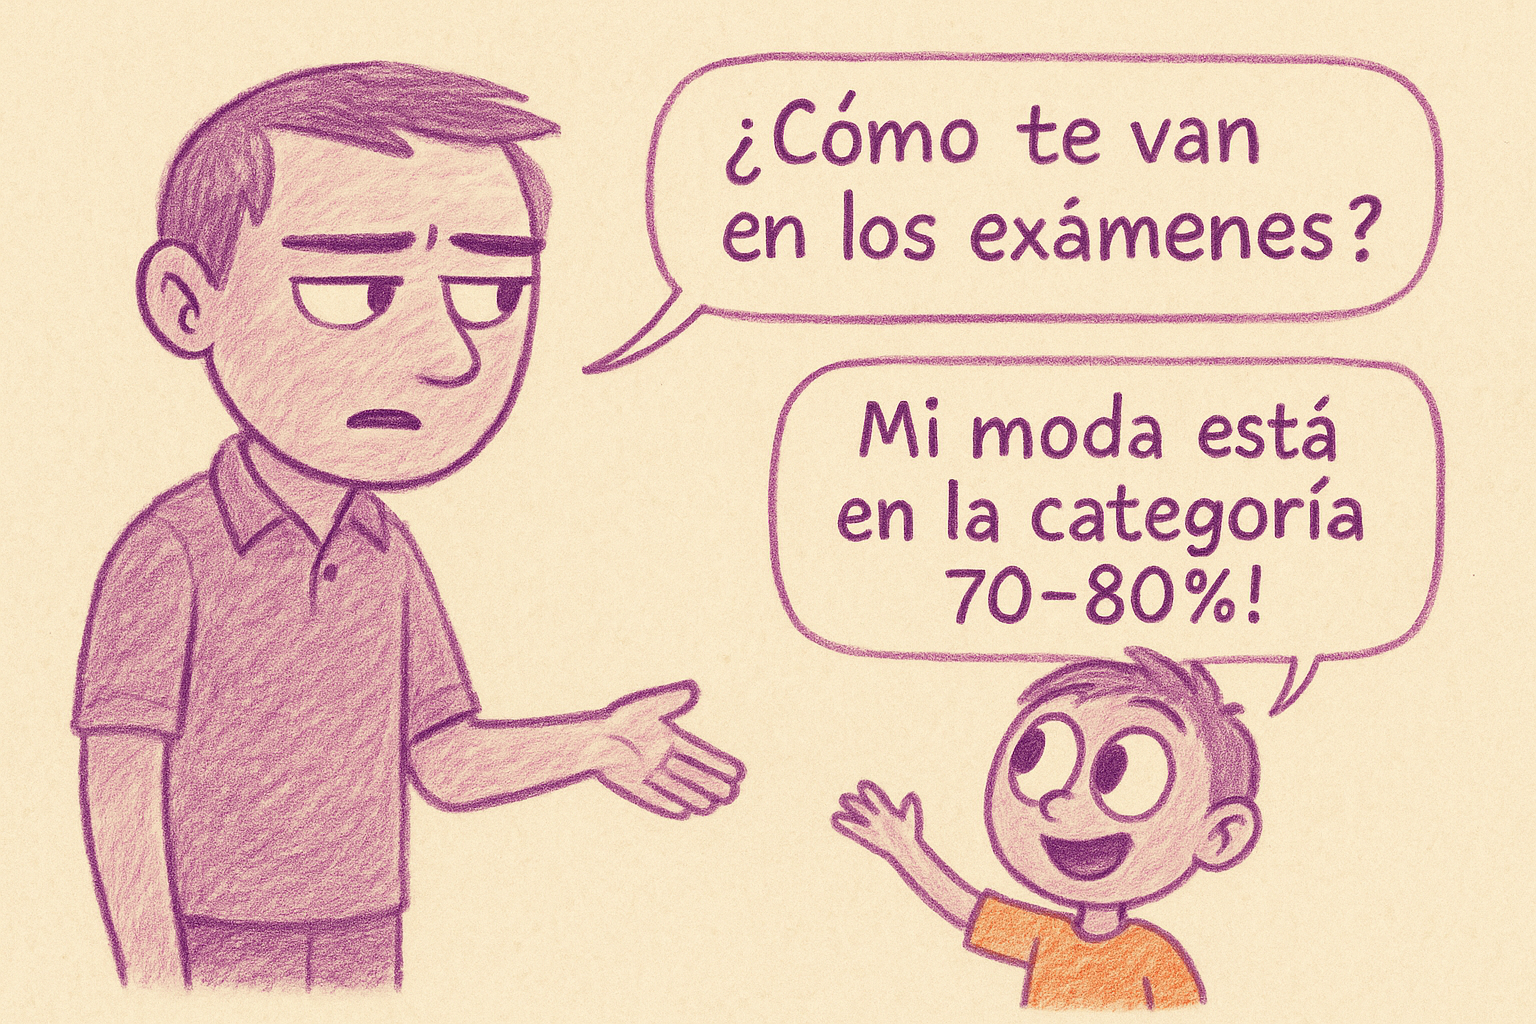
\includegraphics[width=3.64583in,height=\textheight,keepaspectratio]{img/moda_1.png}
\end{center}

\begin{center}
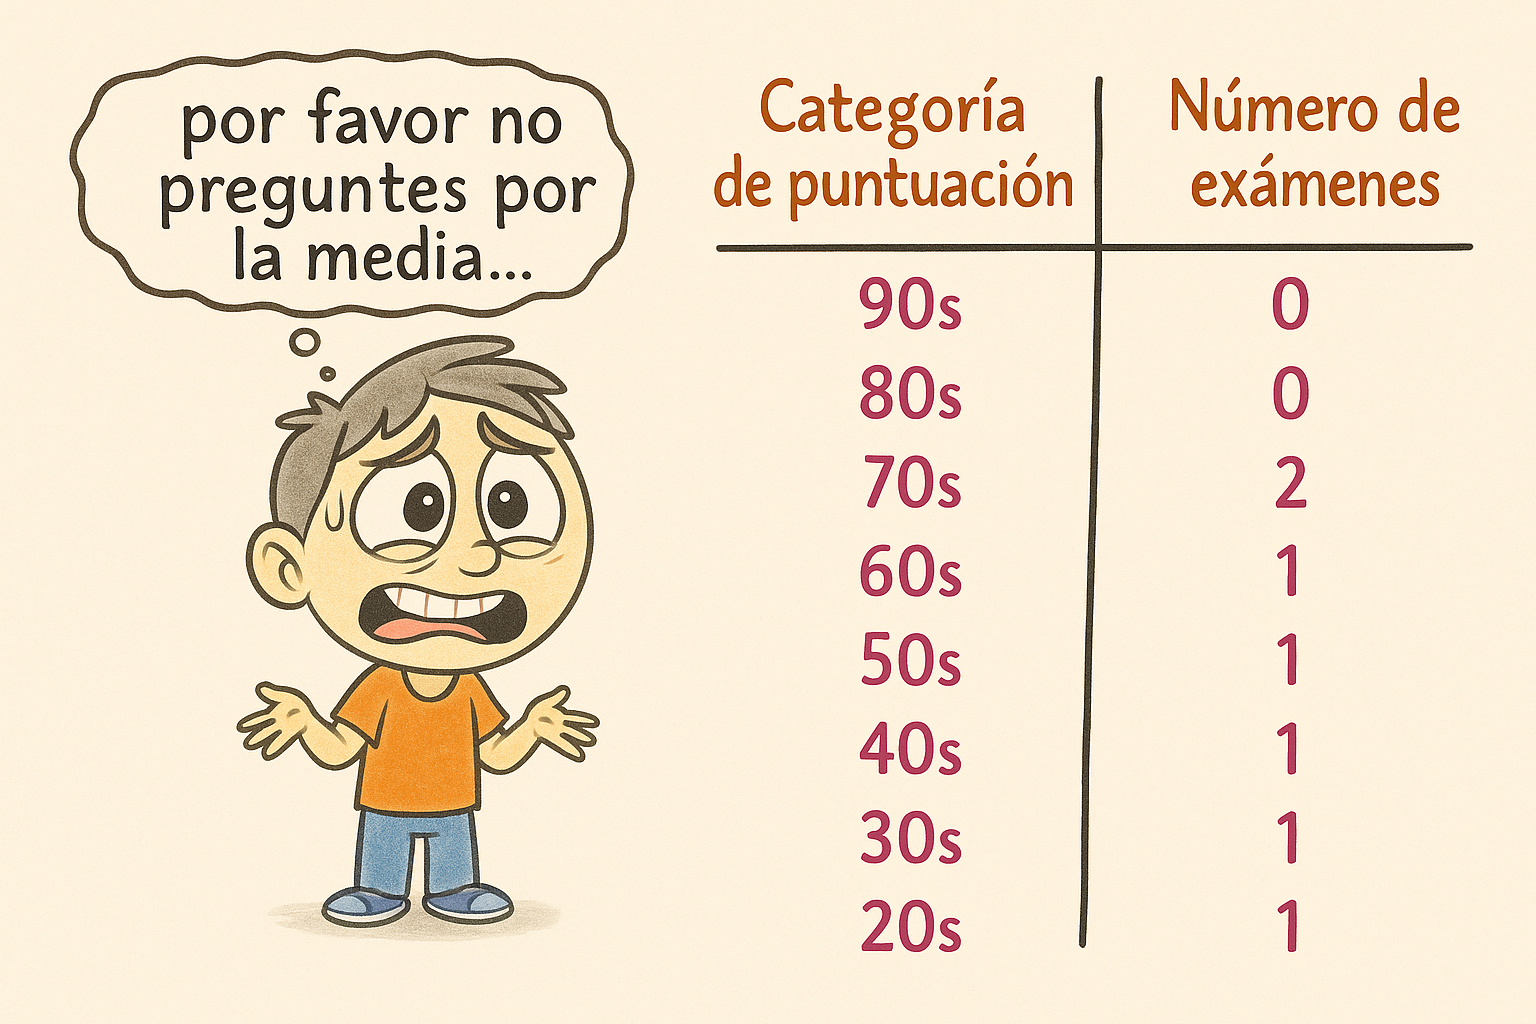
\includegraphics[width=3.64583in,height=\textheight,keepaspectratio]{img/moda_2.png}
\end{center}

\section{Medidas de Variación}\label{medidas-de-variaciuxf3n}

Las medidas de variación nos ayudan a entender qué tan diferentes o
dispersos están los datos entre sí. Es decir, nos dicen si las opiniones
o valores están muy juntos o muy separados.

\subsection{Rango}\label{rango}

Las medidas de variación nos ayudan a entender qué tan diferentes o
dispersos están los datos entre sí. Es decir, nos dicen si las opiniones
o valores están muy juntos o muy separados.

Por ejemplo, si las calificaciones en tu restaurante van desde 2 hasta
5, el rango sería:

\begin{tcolorbox}[enhanced jigsaw, arc=.35mm, leftrule=.75mm, opacityback=0, left=2mm, breakable, colframe=quarto-callout-tip-color-frame, toprule=.15mm, colback=white, bottomrule=.15mm, rightrule=.15mm]
\begin{minipage}[t]{5.5mm}
\textcolor{quarto-callout-tip-color}{\faLightbulb}
\end{minipage}%
\begin{minipage}[t]{\textwidth - 5.5mm}

\[
\text{Rango} = 5 - 2 = 3
\]

\end{minipage}%
\end{tcolorbox}

Esto nos dice que las opiniones varían en un rango de 3 puntos, desde
una calificación baja hasta una alta.

Su principal ventaja es su simplicidad, da una idea rápida del ``ancho''
del conjunto de datos.

Pero su debilidad es igual de clara, solo considera los valores
extremos, ignorando por completo todos los datos intermedios.

Miremos un ejemplo de un rango que da una impresión incorrecta:

\begin{center}
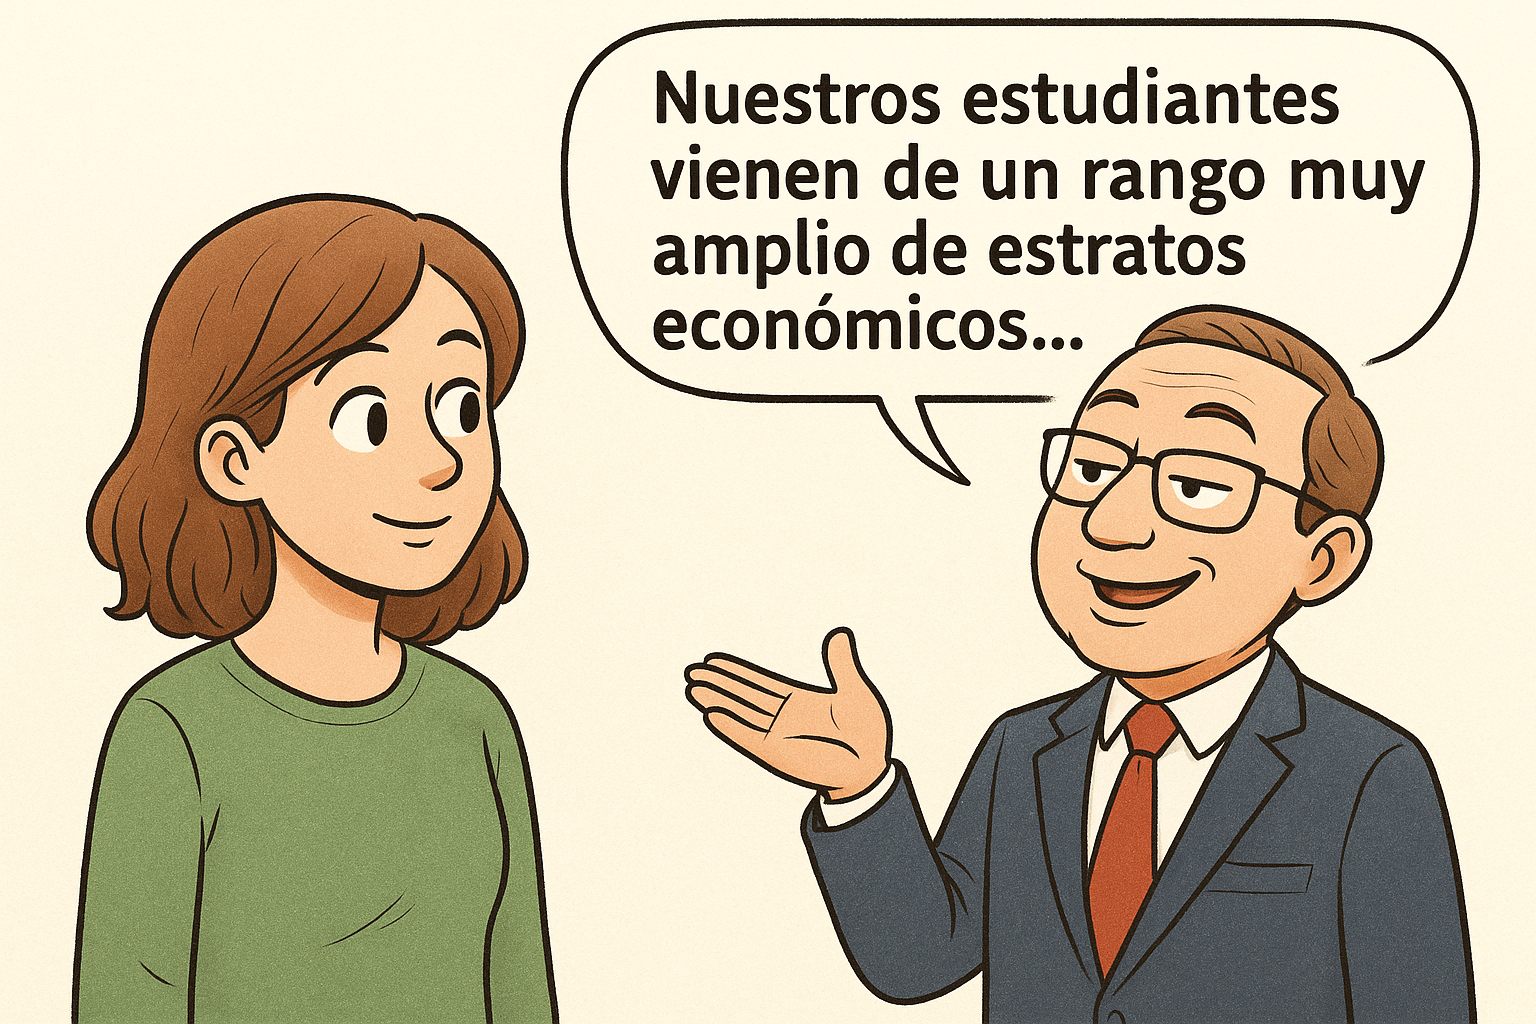
\includegraphics[width=3.64583in,height=\textheight,keepaspectratio]{img/rango_1.png}
\end{center}

\begin{center}
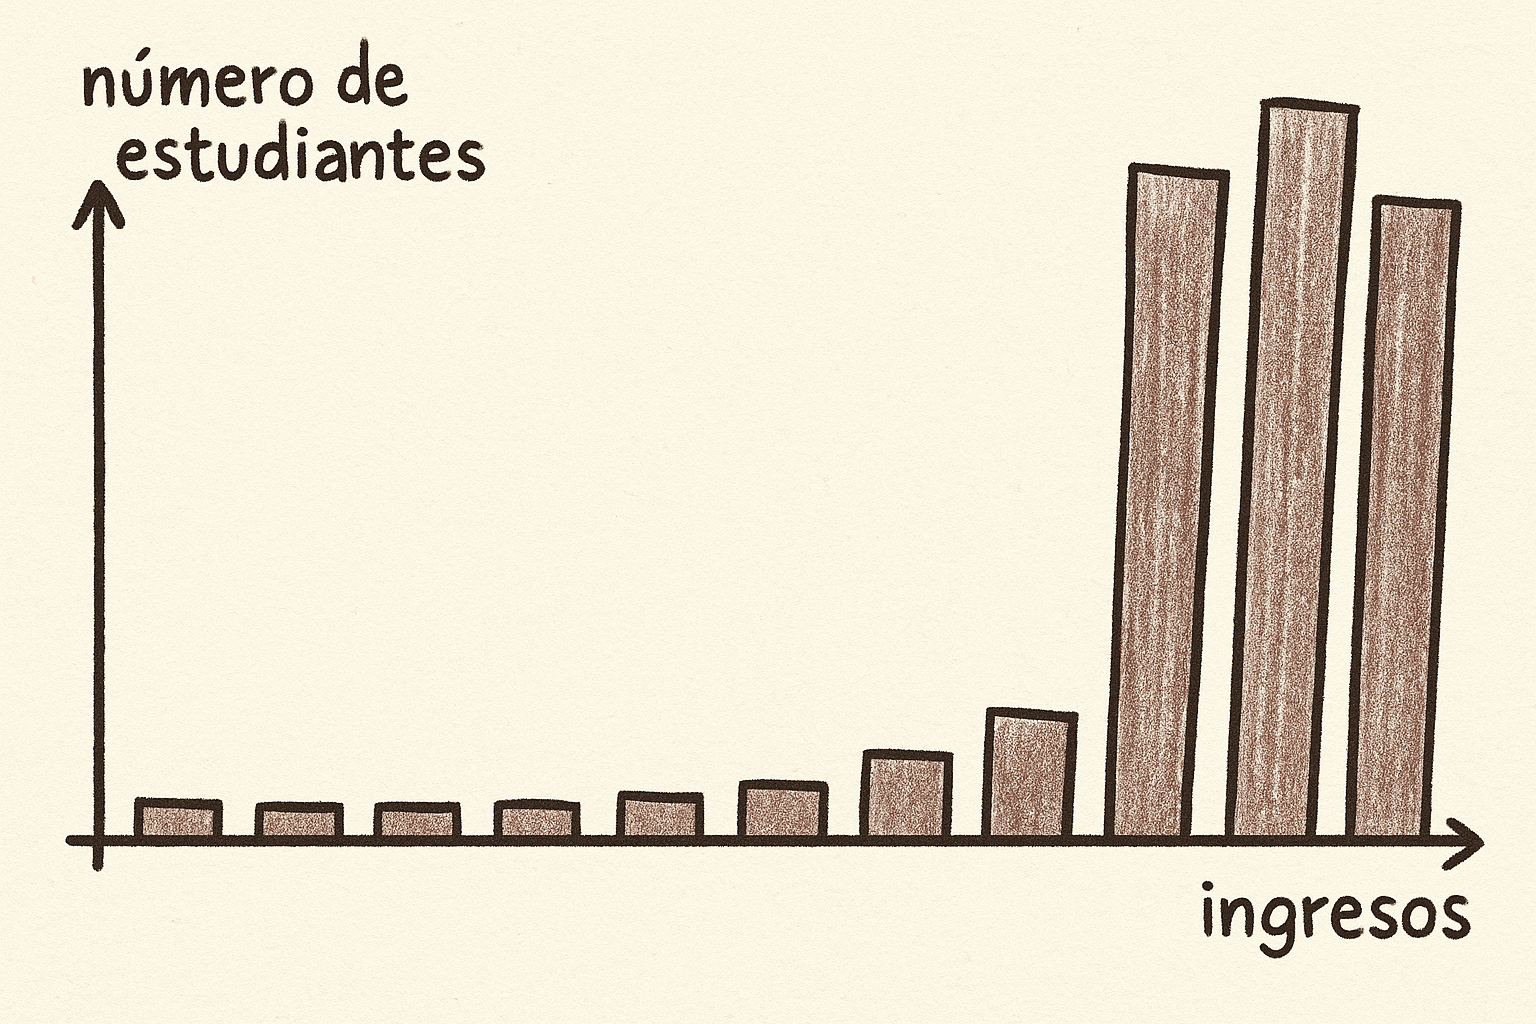
\includegraphics[width=3.64583in,height=\textheight,keepaspectratio]{img/rango_2.png}
\end{center}

\subsection{Varianza y Desviación
Estándar}\label{varianza-y-desviaciuxf3n-estuxe1ndar}

La varianza y la desviación estándar son herramientas que nos ayudan a
entender qué tan dispersos están los datos con respecto a su media.

Imagina que tienes varios números y quieres saber si están todos cerca
del promedio o si están muy separados entre sí.

Para entender qué tan dispersas están las calificaciones de tus clientes
respecto al promedio, usamos dos medidas fundamentales: la
\textbf{varianza} y la \textbf{desviación estándar}:

\begin{itemize}
\tightlist
\item
  Una desviación estándar baja significa que los datos están cerca del
  promedio.
\item
  Una alta desviación estándar indica mucha dispersión.
\end{itemize}

\begin{tcolorbox}[enhanced jigsaw, arc=.35mm, leftrule=.75mm, opacityback=0, left=2mm, breakable, colframe=quarto-callout-tip-color-frame, toprule=.15mm, colback=white, bottomrule=.15mm, rightrule=.15mm]
\begin{minipage}[t]{5.5mm}
\textcolor{quarto-callout-tip-color}{\faLightbulb}
\end{minipage}%
\begin{minipage}[t]{\textwidth - 5.5mm}

Si quisieras ``cocinar'' la varianza en tu propia cocina, la receta
sería así:

\begin{enumerate}
\def\labelenumi{\arabic{enumi}.}
\tightlist
\item
  \textbf{Encuentra la media} de todas las calificaciones.\\
\item
  \textbf{Calcula qué tan lejos está cada calificación de esa media} (la
  diferencia entre cada calificación y la media).\\
\item
  \textbf{Eleva al cuadrado cada una de esas diferencias} para evitar
  que se cancelen y para dar más peso a las diferencias grandes.\\
\item
  \textbf{Suma todas esas diferencias al cuadrado y calcula el promedio}
  dividiendo entre el número de calificaciones menos uno.
\end{enumerate}

\end{minipage}%
\end{tcolorbox}

Matemáticamente, si tienes ( n ) calificaciones ( x\_1, x\_2, \ldots,
x\_n ) y la media ( \bar\{x\} ), la varianza se calcula así:

\begin{tcolorbox}[enhanced jigsaw, arc=.35mm, leftrule=.75mm, opacityback=0, left=2mm, breakable, colframe=quarto-callout-tip-color-frame, toprule=.15mm, colback=white, bottomrule=.15mm, rightrule=.15mm]
\begin{minipage}[t]{5.5mm}
\textcolor{quarto-callout-tip-color}{\faLightbulb}
\end{minipage}%
\begin{minipage}[t]{\textwidth - 5.5mm}

\[
\text{Varianza} = s^2 = \frac{1}{n-1} \sum_{i=1}^n (x_i - \bar{x})^2
\]

\end{minipage}%
\end{tcolorbox}

Pero como la varianza está al cuadrado, no es fácil interpretarla
directamente, pues sus unidades no son las mismas que las de las
calificaciones. Por eso usamos la \textbf{desviación estándar}, que es
la raíz cuadrada de la varianza y nos da una medida en las mismas
unidades originales.

\begin{tcolorbox}[enhanced jigsaw, arc=.35mm, leftrule=.75mm, opacityback=0, left=2mm, breakable, colframe=quarto-callout-tip-color-frame, toprule=.15mm, colback=white, bottomrule=.15mm, rightrule=.15mm]
\begin{minipage}[t]{5.5mm}
\textcolor{quarto-callout-tip-color}{\faLightbulb}
\end{minipage}%
\begin{minipage}[t]{\textwidth - 5.5mm}

\[
\text{Desviación Estándar} = s = \sqrt{s^2}
\]

\end{minipage}%
\end{tcolorbox}

Por ejemplo, si las calificaciones fueron: 4, 5, 3, 4 y 5, la media es:

\begin{tcolorbox}[enhanced jigsaw, arc=.35mm, leftrule=.75mm, opacityback=0, left=2mm, breakable, colframe=quarto-callout-tip-color-frame, toprule=.15mm, colback=white, bottomrule=.15mm, rightrule=.15mm]
\begin{minipage}[t]{5.5mm}
\textcolor{quarto-callout-tip-color}{\faLightbulb}
\end{minipage}%
\begin{minipage}[t]{\textwidth - 5.5mm}

\[
\bar{x} = \frac{4 + 5 + 3 + 4 + 5}{5} = 4.2
\]

\end{minipage}%
\end{tcolorbox}

Luego, calculamos la varianza:

\begin{tcolorbox}[enhanced jigsaw, arc=.35mm, leftrule=.75mm, opacityback=0, left=2mm, breakable, colframe=quarto-callout-tip-color-frame, toprule=.15mm, colback=white, bottomrule=.15mm, rightrule=.15mm]
\begin{minipage}[t]{5.5mm}
\textcolor{quarto-callout-tip-color}{\faLightbulb}
\end{minipage}%
\begin{minipage}[t]{\textwidth - 5.5mm}

\[
s^2 = \frac{(4 - 4.2)^2 + (5 - 4.2)^2 + (3 - 4.2)^2 + (4 - 4.2)^2 + (5 - 4.2)^2}{4} = 0.7
\]

\end{minipage}%
\end{tcolorbox}

Y finalmente, la desviación estándar es:

\begin{tcolorbox}[enhanced jigsaw, arc=.35mm, leftrule=.75mm, opacityback=0, left=2mm, breakable, colframe=quarto-callout-tip-color-frame, toprule=.15mm, colback=white, bottomrule=.15mm, rightrule=.15mm]
\begin{minipage}[t]{5.5mm}
\textcolor{quarto-callout-tip-color}{\faLightbulb}
\end{minipage}%
\begin{minipage}[t]{\textwidth - 5.5mm}

\[
s = \sqrt{0.7} \approx 0.84
\]

\end{minipage}%
\end{tcolorbox}

Esto significa que, en promedio, las calificaciones se alejan de la
media en aproximadamente 0.84 puntos.

A diferencia del rango, que solo considera los valores más extremos, la
varianza y la desviación estándar toman en cuenta todos los datos. Por
eso ofrecen una visión más completa de la dispersión. Sin embargo,
también tienen una desventaja: si hay un solo valor muy alejado (un
valor extremo), puede aumentar mucho la varianza, aunque la mayoría de
los datos estén cerca de la media. Mira el ejemplo a continuación, para
entenderlo mejor:

\begin{center}
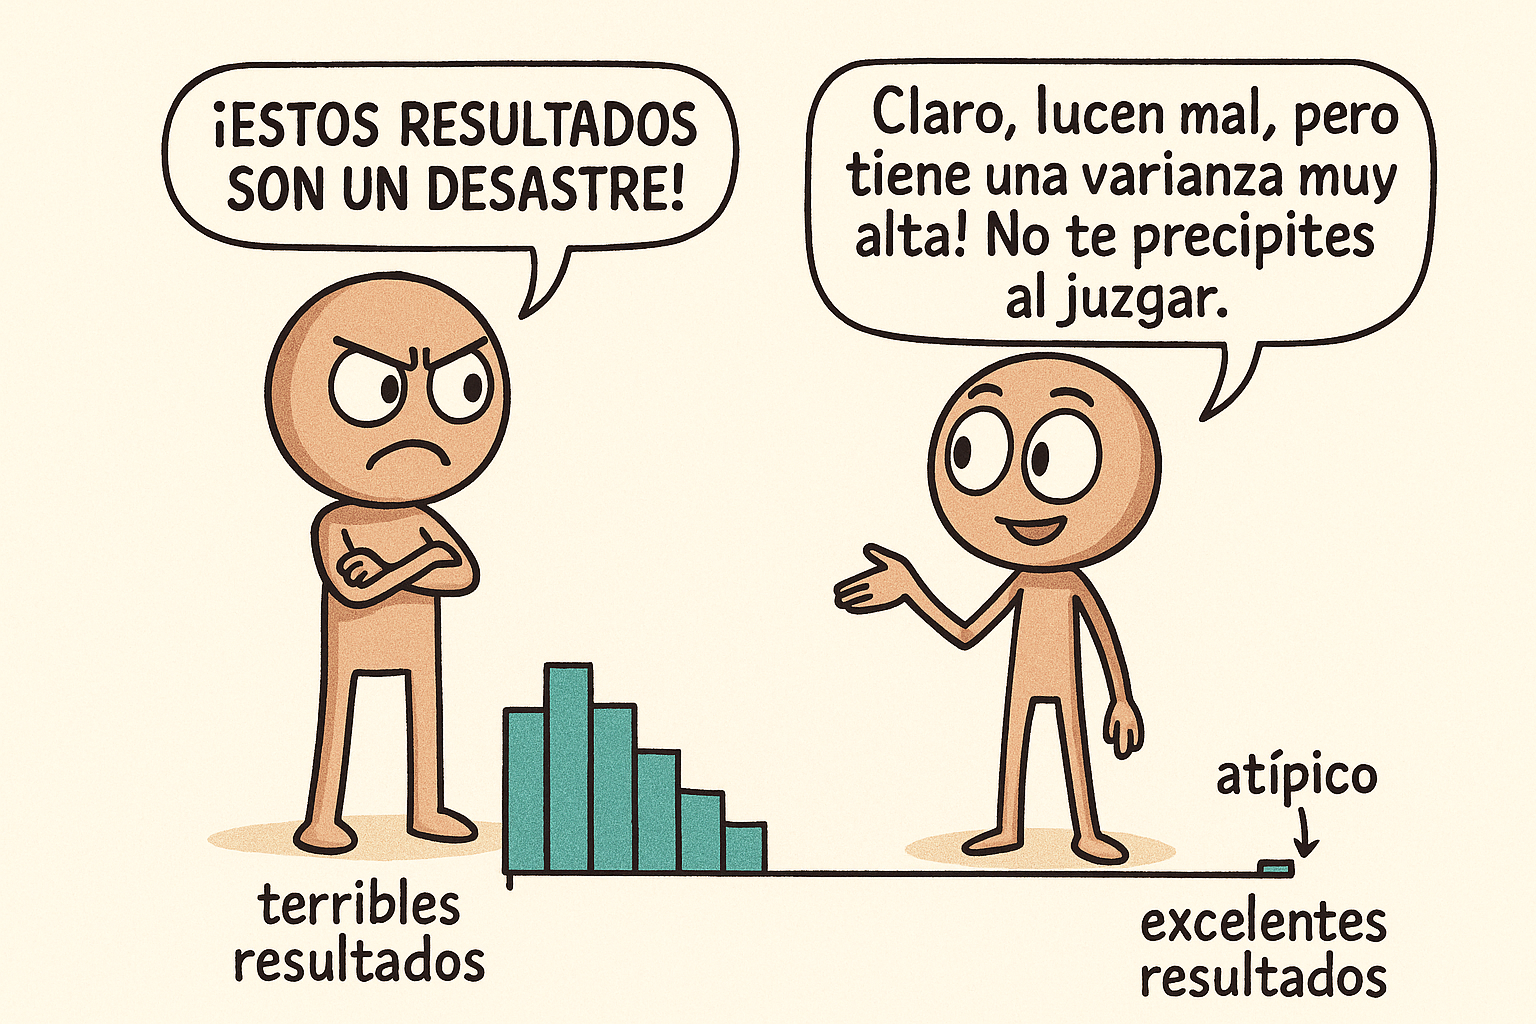
\includegraphics[width=3.64583in,height=\textheight,keepaspectratio]{img/varianza_1.png}
\end{center}

\subsection{Percentil, Cuartiles}\label{percentil-cuartiles}

Imagina que quieres saber cómo se comparan las calificaciones de tus
clientes con todas las demás. Los \textbf{percentiles} nos ayudan a
entender la posición relativa de una calificación dentro del grupo.

Un percentil nos dice qué porcentaje de las calificaciones está por
debajo de cierto valor. Por ejemplo, el \textbf{percentil 25} indica el
punto bajo el cual se encuentra el 25\% de las calificaciones más bajas.

Si una calificación está en el percentil 25, significa que el 25\% de
los clientes dio una calificación igual o menor que esa, y el 75\% dio
una calificación más alta.

Esto es útil para entender la posición relativa de una calificación sin
que las opiniones muy bajas o muy altas influyan demasiado.

Sin embargo, los percentiles \textbf{no nos dicen qué tan separados
están los datos ni qué tan extremos son esos valores.}

Los \textbf{cuartiles} son un tipo especial de percentiles que dividen
las calificaciones en cuatro grupos iguales, cada uno con el 25\% de las
opiniones.

\begin{itemize}
\tightlist
\item
  El \textbf{primer cuartil (Q1)} es igual al percentil 25.\\
\item
  El \textbf{segundo cuartil (Q2)} es la mediana, el punto medio
  (percentil 50).\\
\item
  El \textbf{tercer cuartil (Q3)} es el percentil 75.
\end{itemize}

Esto permite resumir cómo se distribuyen las calificaciones y saber en
qué grupo se ubica cada opinión, incluso si hay calificaciones muy bajas
o muy altas.

\subsection{Rango Intercuartílico
(RIC)}\label{rango-intercuartuxedlico-ric}

Para entender mejor cómo varían las calificaciones en la parte central
de los datos, usamos el \textbf{Rango Intercuartílico}, o \textbf{RIC},
que es la diferencia entre el tercer cuartil y el primer cuartil:

\begin{tcolorbox}[enhanced jigsaw, arc=.35mm, leftrule=.75mm, opacityback=0, left=2mm, breakable, colframe=quarto-callout-tip-color-frame, toprule=.15mm, colback=white, bottomrule=.15mm, rightrule=.15mm]
\begin{minipage}[t]{5.5mm}
\textcolor{quarto-callout-tip-color}{\faLightbulb}
\end{minipage}%
\begin{minipage}[t]{\textwidth - 5.5mm}

\[
RIC = Q3 - Q1
\]

\end{minipage}%
\end{tcolorbox}

El RIC mide la dispersión del 50\% central de las calificaciones,
ignorando las opiniones más bajas y más altas que podrían ser atípicas.

Por ejemplo, si el primer cuartil es 3.5 y el tercer cuartil es 4.5, el
RIC sería:

\begin{tcolorbox}[enhanced jigsaw, arc=.35mm, leftrule=.75mm, opacityback=0, left=2mm, breakable, colframe=quarto-callout-tip-color-frame, toprule=.15mm, colback=white, bottomrule=.15mm, rightrule=.15mm]
\begin{minipage}[t]{5.5mm}
\textcolor{quarto-callout-tip-color}{\faLightbulb}
\end{minipage}%
\begin{minipage}[t]{\textwidth - 5.5mm}

\[
RIC = 4.5 - 3.5 = 1.0
\]

\end{minipage}%
\end{tcolorbox}

Esto indica que la mitad central de las calificaciones está dentro de un
rango de 1 punto, mostrando cuán consistentes son las opiniones
principales.

El RIC es muy útil porque, a diferencia del rango total, \textbf{no se
ve afectado por calificaciones extremas} y nos da una idea clara de la
variabilidad donde está la mayoría de los datos.

\subsection{Diagrama de Caja y Brazos
(Boxplot)}\label{diagrama-de-caja-y-brazos-boxplot}

Para visualizar fácilmente la distribución de las calificaciones de tus
clientes, usamos el \textbf{diagrama de caja y brazos}, también conocido
como \textbf{boxplot}.

Este gráfico muestra en una caja la parte central de los datos, desde el
primer cuartil (Q1) hasta el tercer cuartil (Q3), con una línea en la
mediana (Q2).

Además, los ``brazos'' o líneas que salen de la caja se extienden hasta
los valores mínimos y máximos dentro de un rango razonable, ayudándonos
a identificar si hay calificaciones atípicas o muy extremas.

Así, con un solo gráfico puedes ver:

\begin{itemize}
\tightlist
\item
  Dónde está la mayoría de las calificaciones (la caja).\\
\item
  La calificación típica (la mediana dentro de la caja).\\
\item
  La dispersión general (la longitud de la caja y brazos).\\
\item
  Valores extremos o posibles opiniones fuera de lo común (puntos fuera
  de los brazos).
\end{itemize}

El diagrama de caja es una herramienta poderosa para resumir y comparar
la distribución de las calificaciones de forma rápida y visual.

Este sería un ejemplo en R:

\begin{verbatim}
Warning: package 'ggthemes' was built under R version 4.3.3
\end{verbatim}

\begin{verbatim}
Warning: package 'viridis' was built under R version 4.3.3
\end{verbatim}

\begin{verbatim}
Loading required package: viridisLite
\end{verbatim}

\begin{center}
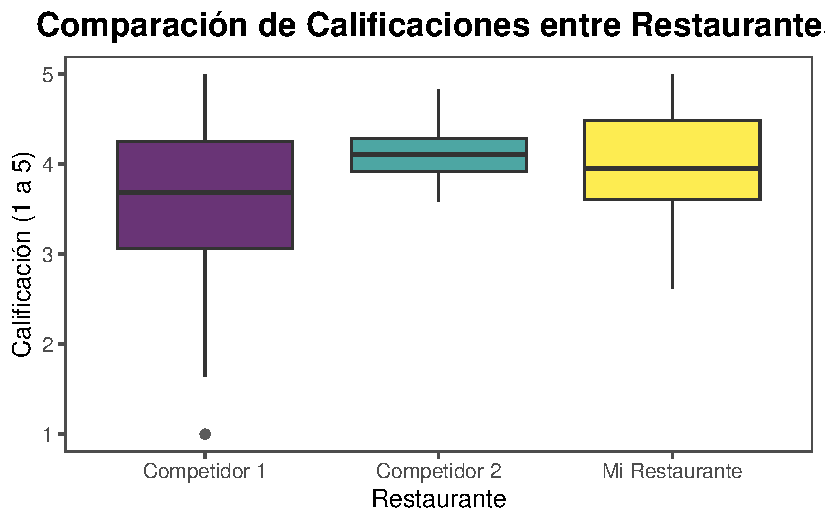
\includegraphics[width=3.64583in,height=\textheight,keepaspectratio]{capitulo3_files/figure-pdf/unnamed-chunk-12-1.pdf}
\end{center}

\section{Medidas de Relación
Lineal}\label{medidas-de-relaciuxf3n-lineal}

Estas nos dicen si dos variables están relacionadas entre sí.

Imagina que además de las calificaciones que dan tus clientes, también
registras cuántas veces visitan tu restaurante al mes. Quieres entender
si estas dos cosas están relacionadas: ¿los clientes que visitan más
tienden a dar mejores calificaciones? ¿O tal vez ocurre lo contrario?

\subsection{Covarianza}\label{covarianza}

La \textbf{covarianza} es una medida que nos indica si dos variables
tienden a subir o bajar juntas.

\begin{itemize}
\tightlist
\item
  Si la covarianza es \textbf{positiva}, significa que cuando una
  variable aumenta, la otra también tiende a aumentar.\\
\item
  Si es \textbf{negativa}, cuando una variable sube, la otra tiende a
  bajar.\\
\item
  Si es cercana a \textbf{cero}, no hay una relación lineal clara entre
  ellas.
\end{itemize}

Sin embargo, la covarianza solo nos dice la dirección de la relación,
pero no qué tan fuerte es, y su valor depende de las unidades de las
variables, lo que dificulta compararla entre diferentes pares de
variables. Es decir, no puedo comparar dos covarianzas de dos variables
distintas.

\subsection{Coeficiente de
Correlación}\label{coeficiente-de-correlaciuxf3n}

Para solucionar esas limitaciones, usamos el \textbf{coeficiente de
correlación}.

Este coeficiente es una versión estandarizada de la covarianza que
siempre toma un valor entre -1 y 1:

\begin{itemize}
\tightlist
\item
  \textbf{1} indica una relación lineal positiva perfecta: a más
  visitas, mejores calificaciones, siempre.\\
\item
  \textbf{-1} indica una relación lineal negativa perfecta: a más
  visitas, peores calificaciones, siempre.\\
\item
  \textbf{0} indica que no hay una relación lineal significativa entre
  las variables.
\end{itemize}

Por ejemplo, un coeficiente de correlación de 0.7 entre visitas y
calificaciones indica una relación positiva fuerte: los clientes que
visitan más suelen estar más satisfechos.

Sin embargo, que haya correlación no implica que una variable
\textbf{cause} la otra, sólo que existe alguna relación la cual incluso
puede ser casualidad no causalidad. Miremos un ejemplo donde correlación
no implica causalidad:

\begin{center}

\includegraphics[width=3.64583in,height=\textheight,keepaspectratio]{img/correlacion_1.png}
\end{center}

\begin{center}
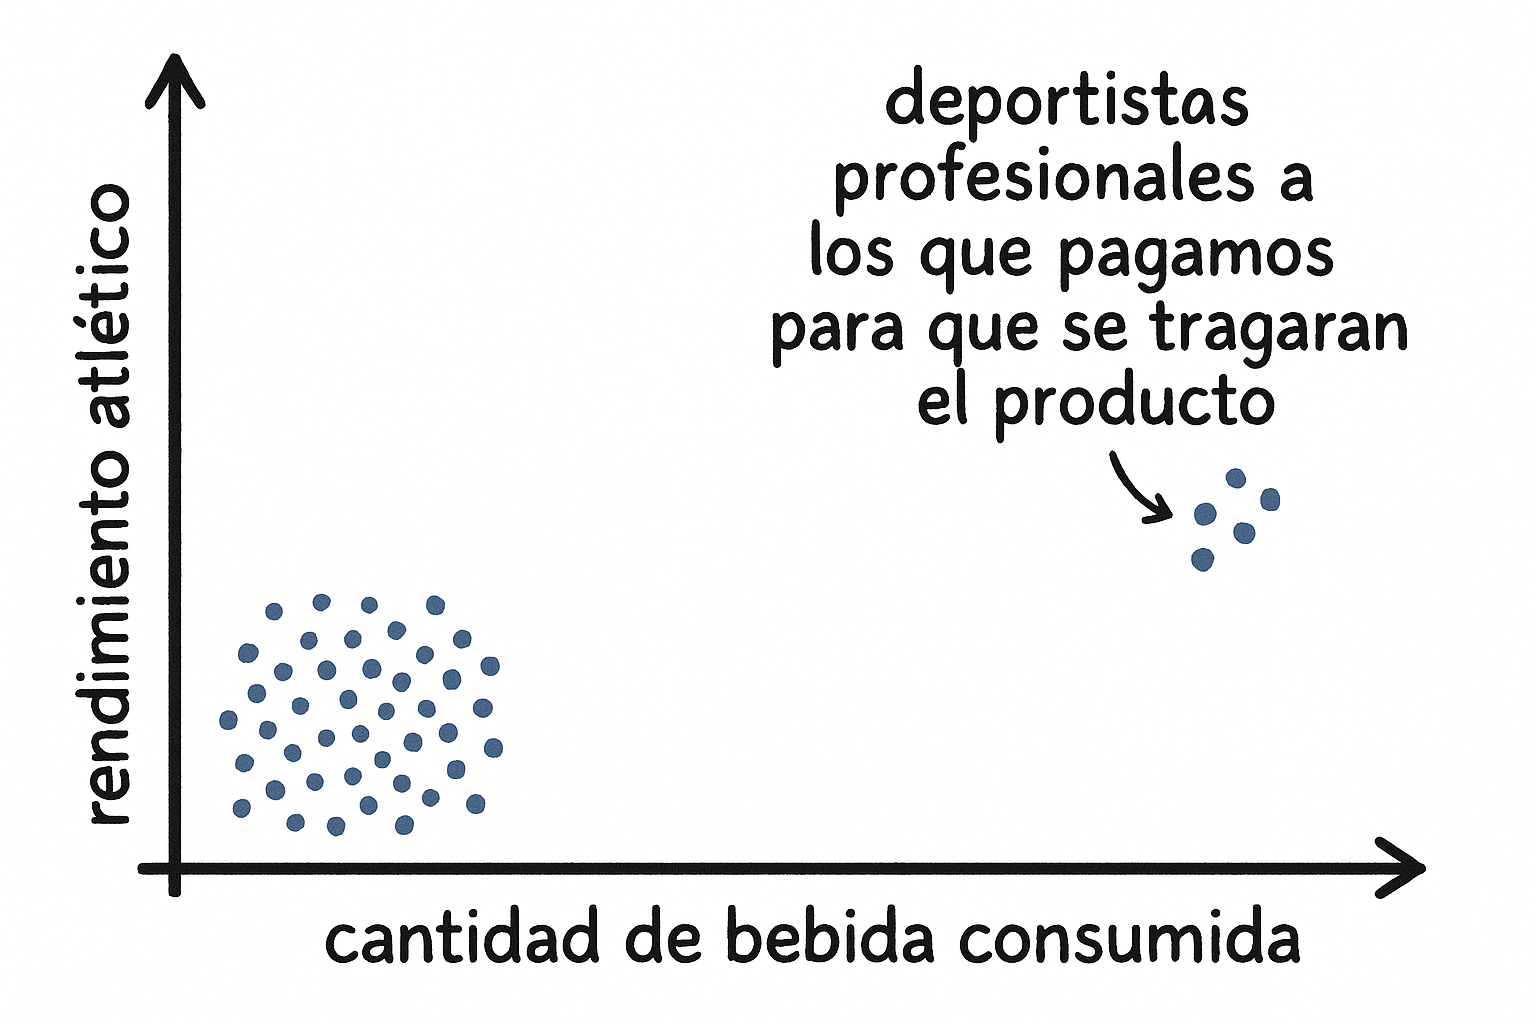
\includegraphics[width=3.64583in,height=\textheight,keepaspectratio]{img/correlacion_2.png}
\end{center}




\end{document}
